\documentclass[12pt,twoside]{article}
%%%%%%%%%%%%%%%%%
%    PACKAGES
%%%%%%%%%%%%%%%%%

% Formatting
\usepackage{setspace} \onehalfspacing % line spacing
\usepackage[top=2.5cm,bottom=2.5cm,inner=4cm,outer=2.5cm]{geometry} % margin sizes
\usepackage[nottoc,notlof,notlot,numbib]{tocbibind} % remove toc from table of contents
\usepackage[none]{hyphenat} % dont hyphenate words
\usepackage{fontspec} \setmainfont{Times New Roman} % set font
\usepackage{enumitem} % reduce spacing for enumerate and itemize
\usepackage{microtype} % fix typing
%\usepackage{lmodern} % font for minted

% Functionality
\usepackage{pdfpages} % include pdf
\usepackage{amsmath} % equations
\usepackage{mathtools} % ceil and floor
\DeclarePairedDelimiter\ceil{\lceil}{\rceil}
\DeclarePairedDelimiter\floor{\lfloor}{\rfloor}
\usepackage{graphicx} % images
\usepackage{float} % figure positioning
\usepackage[hidelinks]{hyperref} % dont highlight links
\usepackage{cleveref} % easy to reference figures
\usepackage{siunitx} % format si units
\usepackage{gensymb} % degree
%\usepackage[cache=false]{minted} % include code
\usepackage[style=ieee]{biblatex} \addbibresource{../zotero.bib} % referencing
%\usepackage{dblfloatfix} % fixes [b] for floats?
\usepackage{subcaption} % subfigures

% Tables
\usepackage{tabularx} % table environment
\usepackage{booktabs} % rules in table
\usepackage{adjustbox} % expand table
\usepackage{makecell} % multi-line cell
\usepackage{pdflscape} % horizontal tables
\usepackage[justification=centering]{caption} % split tables

%%%%%%%%%%%%%%%%%
%    COMMANDS
%%%%%%%%%%%%%%%%%

\raggedbottom % allow pages to end early
\pdfvariable minorversion 7 % updated pdf version
\setlength\parindent{5mm} % change indent size

% change section/subsection title font size to 12
\usepackage{sectsty}
\sectionfont{\fontsize{12}{10}\selectfont}
\subsectionfont{\fontsize{12}{10}\selectfont}
\subsubsectionfont{\fontsize{12}{10}\selectfont}

% change spacing before & after headings
\usepackage{titlesec}
\titlespacing*{\section}{0pt}{24pt}{12pt} % left, before, after
\titlespacing*{\subsection}{0pt}{24pt}{12pt}
\titlespacing*{\subsubsection}{0pt}{24pt}{12pt}

% change spacing around captions and equations
\setlength{\abovecaptionskip}{12pt}
\setlength{\abovedisplayskip}{18pt}
\setlength{\belowdisplayskip}{18pt}
\setlength{\abovedisplayshortskip}{18pt}
\setlength{\belowdisplayshortskip}{18pt}

% "this page left blank"
\newcommand*{\blankpage}{%
\vspace*{\fill}
{\centering \textbf{THIS PAGE INTENTIONALLY LEFT BLANK} \par}
\vspace{\fill}}
\makeatletter
\renewcommand*{\cleardoublepage}{\clearpage\if@twoside \ifodd\c@page\else
\blankpage
\newpage
\if@twocolumn\hbox{}\newpage\fi\fi\fi}
\makeatother

% improve float placement
\setcounter{bottomnumber}{1}
\renewcommand\bottomfraction{10.0}


\begin{document}

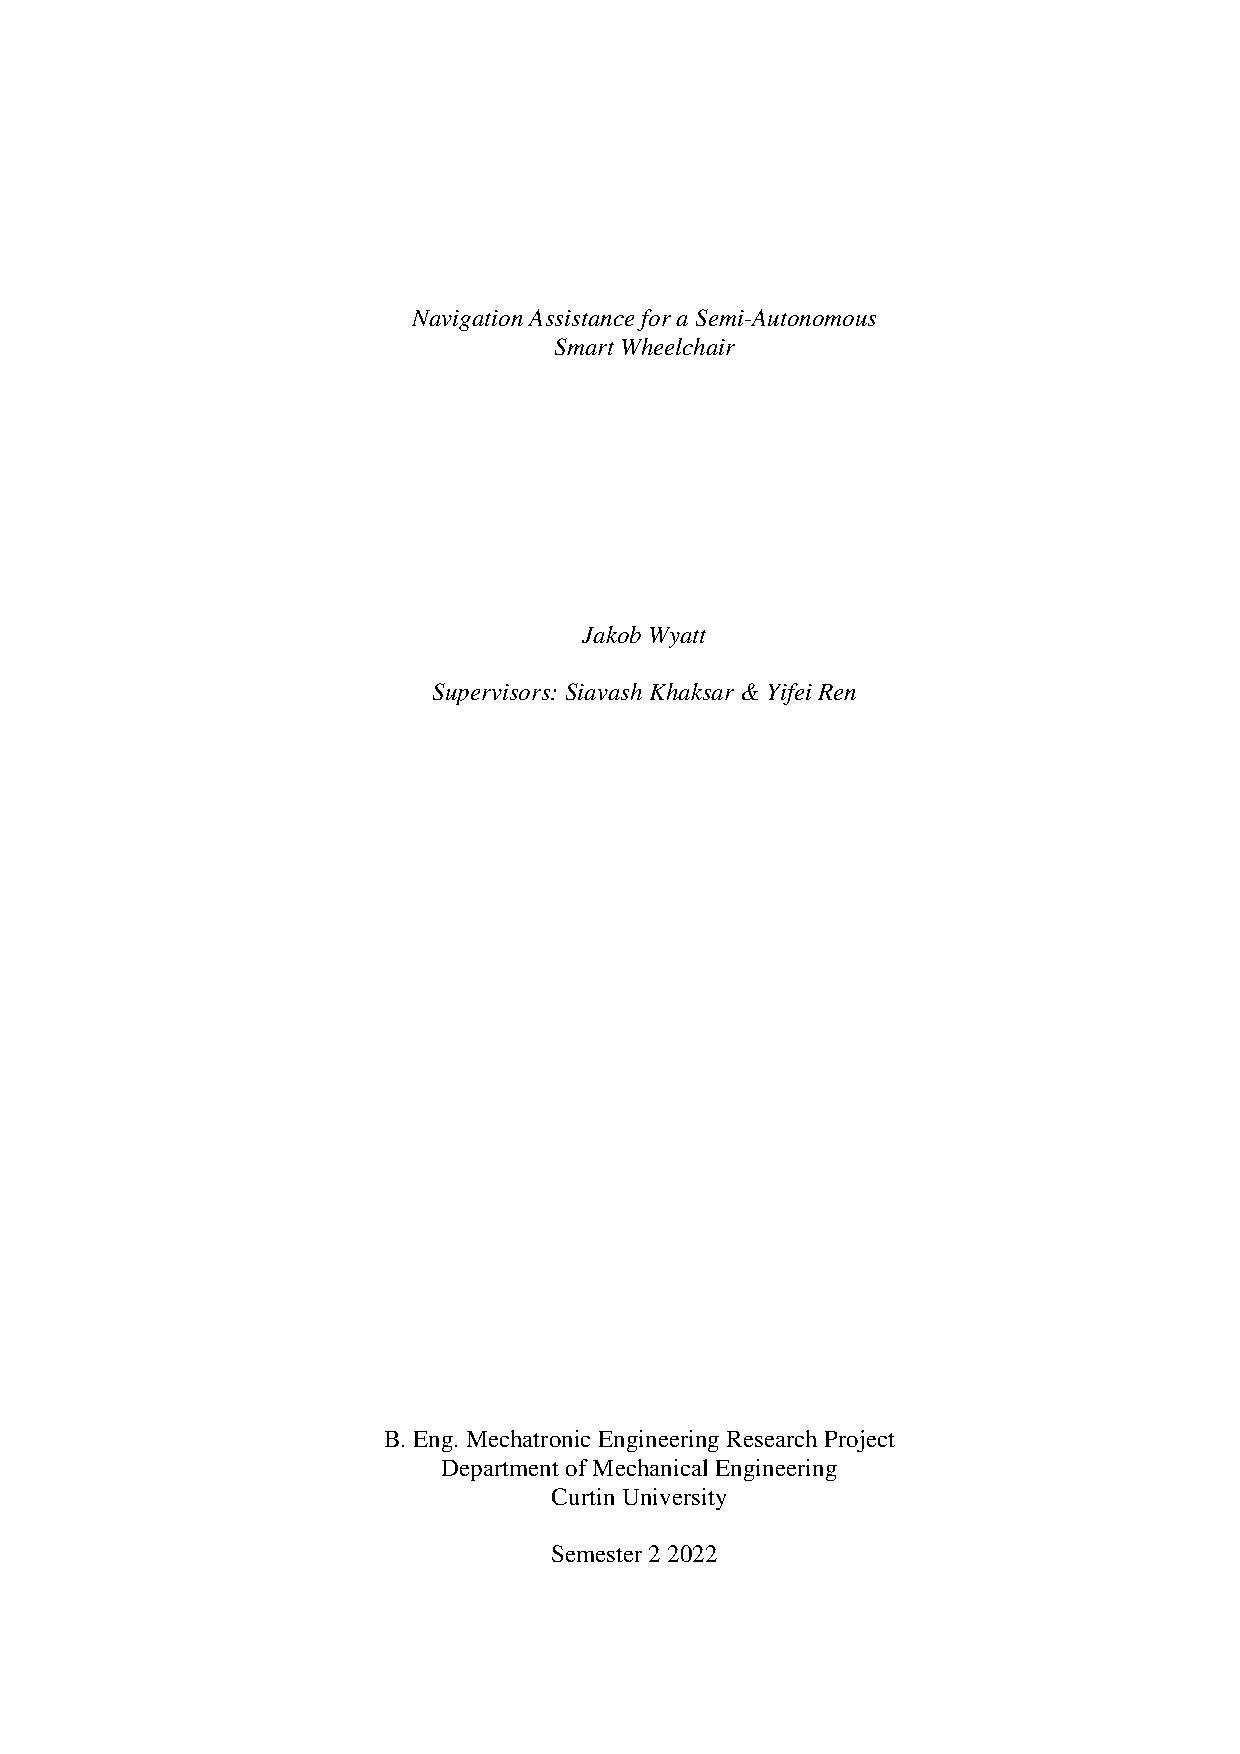
\includepdf{ThesisTitle.pdf}
\thispagestyle{empty}\null\clearpage

\includepdf{ThesisLetter.pdf}
\thispagestyle{empty}\null\clearpage

\pagenumbering{roman}
\section*{ACKNOWLEDGEMENTS}
The author wishes to thank Glide for providing a powered wheelchair to the research team.
% TODO include other acknowledgements
\cleardoublepage

\section*{ABSTRACT}
This progress report involves the identification and definition of the core thesis problem;
creating a semi-autonomous wheelchair that prioritises user safety and independence.
A literature review details prior work in this field, and identifies potential algorithms
for scene recognition and assistive control. Additionally, the literature review identifies and evaluates
sensors that could be used to perceive the wheelchairs environment.

A preliminary wheelchair driving video dataset has been collected around Curtin university.
This dataset has been used to evaluate algorithms such as YOLOv5, DeepLabv3, and Hybridnet on
the problem of scene recognition, with promising results. VFH+ has been evaluated as an assistive
control algorithm after being implemented in MATLAB. Additionally, sensors and hardware to be used
alongside the wheelchair have been identified and evaluated.

The methodology and technical roadmap of this project have been planned, and future work identified (to be completed
next semester). This involves the collection of a second dataset using the final sensors, retraining of
scene recognition models, and final integration of the semi-autonomous system with the wheelchair.

\cleardoublepage

\section*{DECLARATION OF PUBLISHED WORKS}
% TODO use format provided by Siavash
I acknowledge that the literature review of this thesis was previously submitted as part of the Progress Report assessment for MXEN4000.
I also acknowledge that this thesis contains no material previously
published by any other person except where due acknowledgment has been made.

\cleardoublepage

\renewcommand{\contentsname}{TABLE OF CONTENTS}
\tableofcontents
\pagebreak
\listoffigures
\listoftables
\cleardoublepage
\pagenumbering{arabic}

\section{INTRODUCTION}
\subsection{Background and Motivation}
Powered wheelchairs have substantially benefited people with mobility challenges.
The use of these wheelchair systems has been shown to improve the user's independence, quality
of life and feeling of well-being \cite{treflerOutcomesWheelchairSystems2004}.
However, this technology can be inaccessible or unsafe for people with vision impairment,
multiple sclerosis, ALS, and cerebral palsy, due to difficulties with environmental perception
or joystick use. A survey of 65 clinicians found that 10-40\% of patients found it impossible or
extremely difficult to use a powered wheelchair \cite{fehrAdequacyPowerWheelchair2000}.

Smart wheelchairs add intelligent sensing and control to an existing powered wheelchair
to avoid obstacles in the environment or navigate the user.
Additionally, a smart wheelchair may include alternative input methods such as
eye gaze \cite{eidNovelEyeGazeControlledWheelchair2016}, head tilt \cite{tomariEnhancingWheelchairControl2014},
and voice recognition \cite{bakouriSteeringRoboticWheelchair2022}.
Fully-autonomous smart wheelchairs move the user from a start pose to an end goal,
and often require a map of the surrounding environment or markers
such as QR codes \cite{habhaAutonomousWheelchairIndoorOutdoor2021}.
Semi-autonomous smart wheelchairs blend input from the user with the control unit
to avoid obstacles and improve safety. Using a smart wheelchair improves the user's
safety and independence; Simpson et al. found that over 61\% of
current wheelchair users would benefit from some smart wheelchair features \cite{simpsonHowManyPeople2008}.

\subsection{Aims}
This research aims to develop a semi-autonomous smart wheelchair system.
This research was done in collaboration with Glide, a WA wheelchair manufacturer,
who has provided an existing powered wheelchair (CentroGlide) to use as a base
for this functionality (\cref{fig:wheelchair}). By developing assistive technology for the wheelchair,
the user is granted greater mobility, confidence, and independence.

The project team comprises multiple engineering project students, researchers, and interns.
This team has worked on many smart wheelchair features, including motor controller design (Kosma Egan),
input controller design (Brian Smith), doorway navigation (Avinash Sudhakaran),
object detection (Krishnadas Suresh), and vehicle transfer (Nicolas Lee).
The specific aim of this thesis is to implement navigation assistance,
which involves both avoiding environmental obstacles such as walls and stairs,
and guiding the user along suitable pathways. If a user were to unintentionally
drive off a pathway, they could encounter a kerb or uneven terrain, which could lead
to a fall.

\pagebreak
\subsection{Problem Definition}
An important requirement of this project is that the user still
has control over their wheelchair and can override any autonomous functionality
if required. If the smart wheelchair system mistakenly detects an obstacle,
the user's mobility should not be compromised.

Another requirement of the system is that any sensors mounted to the wheelchair
should not impede the user's comfort or the wheelchair's manoeuvrability.
Many wheelchair users have specific requirements for wheelchair seat adjustments
to avoid pressure sores and discomfort. \Cref{fig:wheelchair} shows the
wheelchair configuration when fully reclined, demonstrating that some sensor mounting locations
are infeasible.

The smart wheelchair system should also be commercially viable - high-cost
components and sensors are infeasible. Internet connectivity should not be a requirement
for the system to operate either - the round trip time required to communicate with a server
could compromise the safety of a user. Because of this, all processing is performed locally
on the wheelchair.

\begin{figure}[b]
    \centering
    \begin{subfigure}{.45\textwidth}
        \centering
        \includegraphics[height=\linewidth,angle=270,origin=c]{images/wheelchair.jpg}
        \caption{Upright}
    \end{subfigure}
    \quad
    \begin{subfigure}{.45\textwidth}
        \centering
        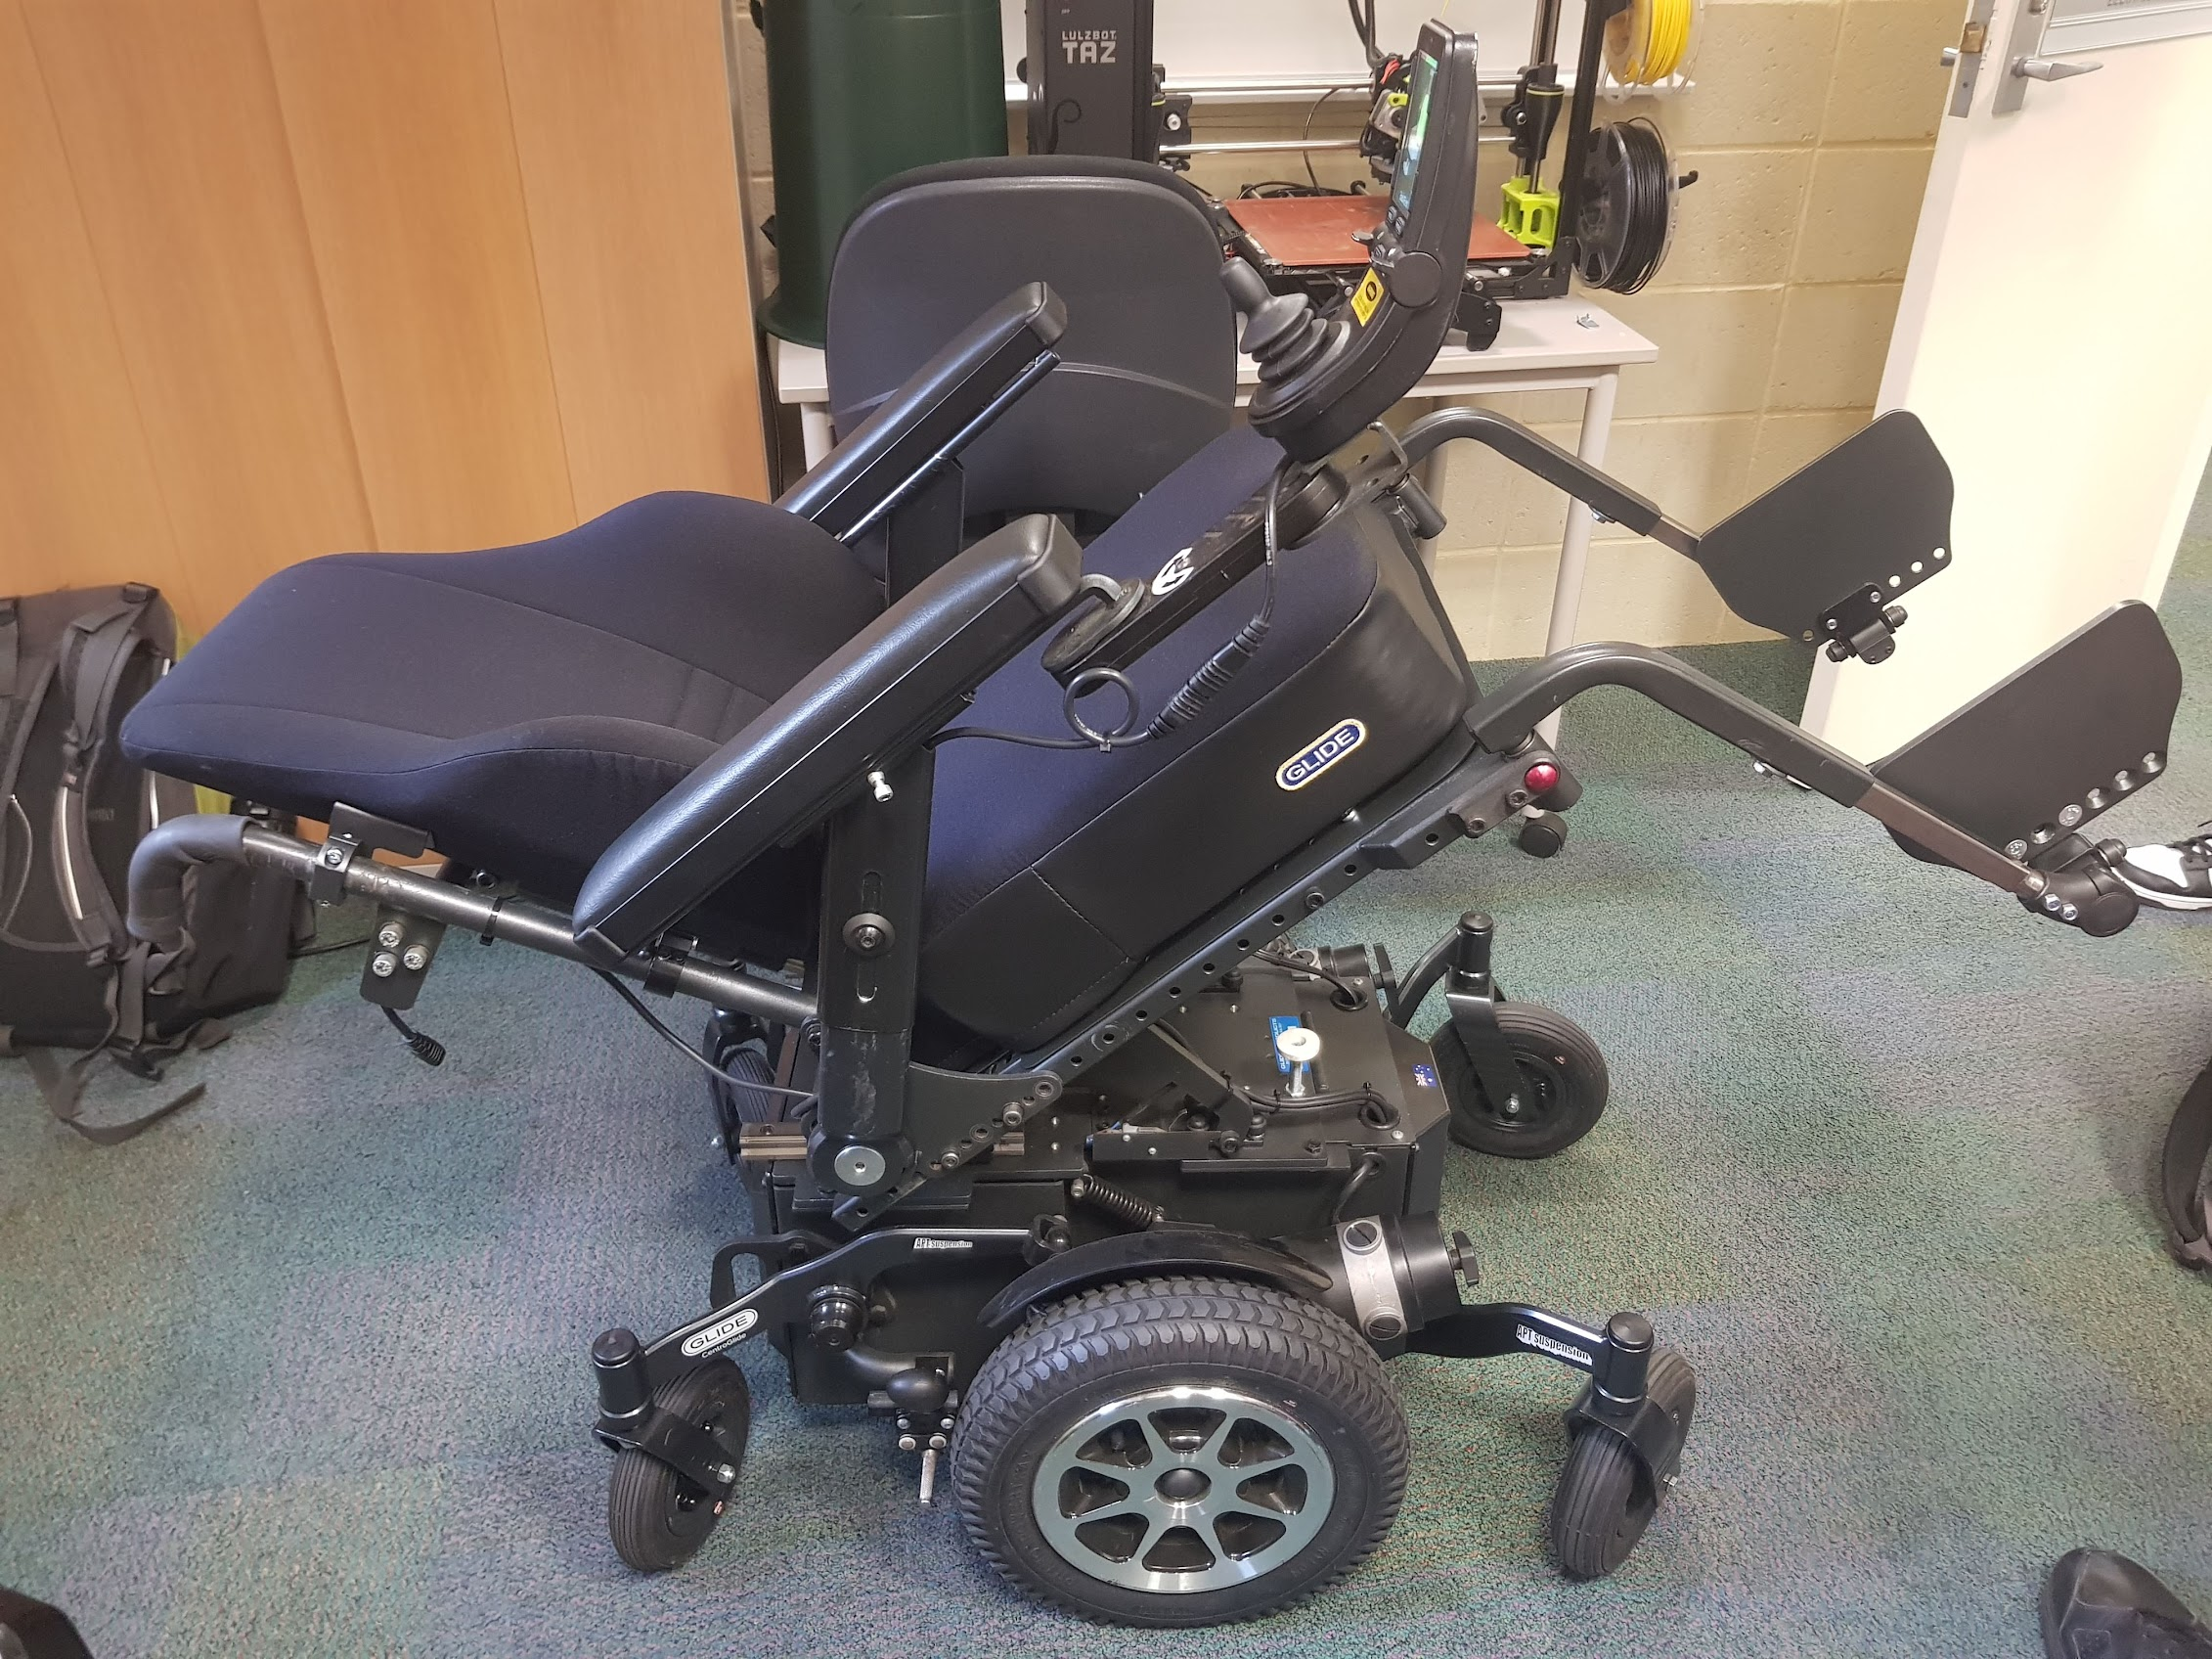
\includegraphics[width=\linewidth]{images/wheelchair_reclined.jpg}
        \caption{Reclined}
    \end{subfigure}
    \caption{CentroGlide wheelchair}
    \label{fig:wheelchair}
\end{figure}

\cleardoublepage

\section{LITERATURE REVIEW}
%Smart wheelchairs are wheelchairs with additional sensors and computers,
%enabling greater usability and safety. This can come in the form of alternative input methods,
%such as eye-gaze tracking \cite{eidNovelEyeGazeControlledWheelchair2016} or using a brain-computer
%interface \cite{kaufmannBraincomputerInterfaceBased2014} to control the wheelchair. For people with vision impairment,
%haptic feedback \cite{kondoNavigationGuidanceControl2008}\cite{vanderpoortenPoweredWheelchairNavigation2012}
%has been used to improve awareness of the surrounding environment and make indoor navigation safer.


\subsection{Sensors and Hardware}
%To perceive the environment, the wheelchair should be fitted with various sensors and
%a compute element to process the sensors output.

\subsubsection{Sensor Types}
Smart wheelchairs have used a varied range of sensor types to perceive the surrounding environment.
RGB-D stereo cameras have been widely used in the field \cite{wangS2P2SelfSupervisedGoalDirected2021}\cite{wangSelfSupervisedDrivableArea2019}\cite{jainAutomatedPerceptionSafe2014},
alongside 2D Lidar \cite{scudellariSelfdrivingWheelchairsDebut2017} and ultrasonic sensors \cite{levineNavChairAssistiveWheelchair1999}.
Self-driving cars built by companies such as Tesla and Waymo
use cameras, mmWave Radar, and 3D Lidar to avoid traffic and pedestrians \cite{karpathyTeslaAIDay2021}.

Selecting a sensor to use is not necessarily an either-or decision. Sensor fusion algorithms such as
the Extended Kalman Filter (EKF) or Unscented Kalman Filter (UKF) \cite{wanUnscentedKalmanFilter2000} allow
outputs from multiple sensors to be used together to improve their accuracy. Additionally, sensors can
be used for different applications on the smart wheelchair - a stereo camera could be used to sense the surrounding environment
while an inertial measurement unit (IMU) could be used for wheelchair odometry.
\Cref{table:sensor_options} compares several available sensor types,
taking into account factors such as resolution, cost, and accuracy.

\begin{table}[H]
    \centering
\begin{adjustbox}{width=\textwidth}
    \begin{tabular}{c c c}
    \toprule
    Sensor & Advantages & Disadvantages \\
    \midrule
    RGB-D Stereo Camera & Very high resolution & Low field of view (FOV) \\
    mmWave Radar & High accuracy & Low resolution \\
    3D Lidar & High resolution and accuracy & Very high cost \\
    2D Lidar & High FOV and accuracy & Only detects obstacles within the same plane \\
    Ultrasonic sensor & Low cost & One-dimensional \\
    \bottomrule
    \end{tabular}
\end{adjustbox}
    \caption{Sensor comparisons}
    \label{table:sensor_options}
\end{table}

% Description of different sensor types?

\subsubsection{RGB-D Cameras}
One advantage RGB-D cameras have over alternative sensors is high RGB resolution,
allowing them to utilise advances in machine learning and computer vision.
Technologies such as Lidar may fail at path detection, as path markings
cannot be detected.

When comparing these cameras, factors such as package size,
field of view, and operating range are important to consider.
Several commercial options are compared in \Cref{table:stereo_camera}
- all of the listed units come with an integrated IMU.

\begin{landscape}
\begin{table}[H]
    \centering
    \begin{tabular}{c c c c c c}
    \toprule
    Name & Type & Cost (AUD)\footnotemark[1] & Dimensions (mm) \\
    \midrule
    Stereolabs Zed Mini \cite{stereolabsZEDMiniCamera2018} & Passive & \$595 & $124.5\times 30.5\times 26.5$ \\
    Stereolabs Zed 2 \cite{stereolabsZEDCameraSDK2019} & Passive & \$670 & $175\times 30\times 33$ \\
    Intel RealSense D455 \cite{intelIntelRealSenseProduct2022} & Active IR (Stereo) & \$595 & $124\times 26\times 29$ \\
    Microsoft Azure Kinect DK \cite{microsoftAzureKinectDK2021} & Active IR (Time of Flight)\footnotemark[2] & \$595 & $103\times 39\times 126$ \\
    \bottomrule
    \end{tabular}
    \caption{Stereo camera options}
    \label{table:stereo_camera}
\end{table}
\addtocounter{table}{-1}
\begin{table}[H]
    \centering
    \begin{tabular}{c c c c c c}
    \toprule
    Name & FOV (Horizontal, Vertical, Depth) & Operating Range (m) \\
    \midrule
    Stereolabs Zed Mini \cite{stereolabsZEDMiniCamera2018} & $90\degree\times 60\degree\times 100\degree$ & 0.1-15\\
    Stereolabs Zed 2 \cite{stereolabsZEDCameraSDK2019} & $110\degree\times 70\degree\times 120\degree$ & 0.3-20 \\
    Intel RealSense D455 \cite{intelIntelRealSenseProduct2022} & $90\degree\times 65\degree\times 87\degree$ & 0.6-6 \\
    Microsoft Azure Kinect DK \cite{microsoftAzureKinectDK2021} & $75\degree\times 65\degree\times 75\degree$ & 0.5-3.86 \\
    \bottomrule
    \end{tabular}
    \captionsetup{list=no}
    \caption{Stereo camera options (continued)}
\end{table}

\begin{table}[H]
    \centering
\begin{adjustbox}{width=1.25\textwidth}
    \begin{tabular}{c c c c c c}
    \toprule
    Name & Cost (AUD)\footnotemark[1] & Release Year & Speed & Power & Notes \\
    \midrule
    Nvidia Jetson Nano \cite{nvidiaJetsonNanoSystemonModule2019} & \$150 & Early 2019 & 0.5 TFLOPS (FP16) & 10 W & - \\
    Nvidia Jetson Xavier NX \cite{nvidiaJetsonXavierNX2019} & \$595 & Late 2019 & 21 TOPS (INT8) & 20 W & - \\
    Nvidia RTX 2080 \cite{nvidiaTuringGPUArchitecture2018} & \$1040 & 2018 & \makecell{80.5 TFLOPS (FP16)\\161.1 TOPS (INT8)} & 215 W & Doesn't include single-board computer \\
    Google Coral Edge TPU \cite{googlecoralCoralDevBoard2020} & \$190 & 2020 & 4 TOPS (INT8) & 2 W & Only supports TensorFlow Lite \\
    \bottomrule
    \end{tabular}
\end{adjustbox}
    \caption{AI accelerator options}
    \label{table:compute_element}
\end{table}
\end{landscape}

\footnotetext[1]{Costs are taken at RRP with an exchange rate of 1 AUD = 0.74 USD}
\footnotetext[2]{The Microsoft Azure Kinect DK has multiple operating modes that trade-off between FOV, operating range, and resolution. The \texttt{NFOV unbinned} mode was compared, which provides good trade-off between operating range and resolution.}

A caveat of the Stereolabs products is that they require a separate CUDA-enabled GPU (manufactured by Nvidia) to generate the point-cloud
and RGB-D image. In contrast, the Kinect DK only requires a CPU for processing, while the Intel RealSense performs processing onboard
and requires a USB-C 3.1 interface to communicate.

\subsubsection{Compute Element}
A compute element inside a semi-autonomous driving system generally consists of several components -
a microcontroller to process user inputs and
send signals to the motors, a general-purpose computer to run pathfinding algorithms and log information,
and an AI accelerator to improve the performance of on-board machine learning (ML) algorithms.

AI accelerators use specialised hardware to perform operations common in ML algorithms (such as matrix multiplication
and convolution) more efficiently than a CPU can. GPUs have been used widely for this application; however, their high
power usage is infeasible for some applications. Embedded AI accelerators aim to provide greater power efficiency
at the cost of specialisation.

Machine learning models often use mixed-precision (FP16) datatypes to store weights while training.
Although improving the model's accuracy, FP16 datatypes are slow to manipulate during inference.
Model quantisation \cite{jacobQuantizationTrainingNeural2017} is a process where this FP16 datatype is replaced with an
INT8 datatype (using a scaling factor and bias) after training.
Quantisation greatly improves speed while only losing a small amount of model accuracy.
For this reason, modern AI accelerators focus on the performance of INT8 operations (TOPS, $10^9$ operations per second),
whereas earlier accelerators state the performance of FP16 operations (TFLOPS, $10^9$ floating-point
operations per second).

The Nvidia Jetson and Google Coral products are both popular options for embedded AI acceleration. These accelerators are compared
in \Cref{table:compute_element} alongside a gaming GPU. 

\pagebreak
\subsection{Scene Understanding}
Scene understanding is a broad field and involves using computer vision methods
on visual or spatial data to gain better knowledge about the surrounding environment.
Convolutional Neural Networks (CNNs) are commonly used for this application, as they
can exploit the local nature of image features to reduce the number of required computations.

\subsubsection{Image Classification}
Image classification is a core problem within this field and involves identifying the subject of an image (such as an animal or object).
AlexNet \cite{krizhevskyImageNetClassificationDeep2012}, based on the earlier digit-recognition CNN LeNet-5
\cite{lecunGradientbasedLearningApplied1998}, was one of the first deep CNNs
applied to this problem. AlexNet was trained on the large ImageNet dataset \cite{jiadengImageNetLargescaleHierarchical2009},
which consists of 15M images and 22K categories,
and achieved an error of only 15.3\% on a 1000 class subset. The underlying architecture uses a series of 5 convolutional
layers and 3 fully connected layers, which can be seen in \cref{fig:alexnet_architecture}.

\begin{figure}[b]
    \centering
    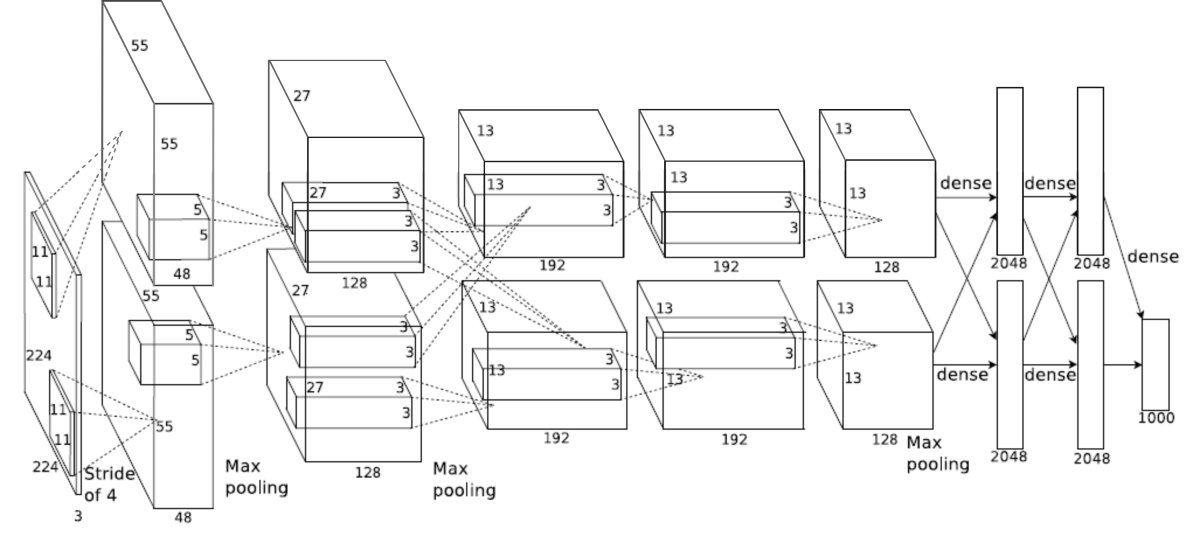
\includegraphics[width=0.8\linewidth]{images/alexnet_architecture.png}
    \caption{Architecture of the AlexNet image classification network. Reproduced from Krizhevsky et al. \cite{krizhevskyImageNetClassificationDeep2012}}
    \label{fig:alexnet_architecture}
\end{figure}

Neural network architectures have become deeper and more accurate over time, enabled by both
growth in computational power and dataset size. VGG-16 \cite{simonyanVeryDeepConvolutional2014}
and GoogLeNet \cite{szegedyGoingDeeperConvolutions2014}
are 16 and 22 layers deep respectively, and approached
human performance on the ImageNet dataset. ResNet \cite{heDeepResidualLearning2016} is up to 156 layers deep,
and exceeds human performance at image classification with an error of 3.57\%.
ResNet uses a 'skipping' architecture to improve network training, where the output of a layer relies directly on
the input of a previous layer.

\subsubsection{Object Localisation}
Object localisation is another core problem within this field, and involves identifying the location of objects within an image as well as classifying them.
Object localisation can be used on a semi-autonomous wheelchair to identify
a pedestrian or obstacle within the environment. R-CNN \cite{girshickRichFeatureHierarchies2013} was one of the
first object classification models which utilised convolutional networks, by identifying potential bounding boxes
and running an image classifier on these bounding boxes. Fast and Faster R-CNN \cite{girshickFastRCNN2015}\cite{renFasterRCNNRealTime2015}
improved the speed of this model by running an image classifier backbone once on the entire image, and using a CNN to improve
the identification of bounding boxes. Pascal VOC \cite{everinghamPascalVisualObject2009} and MS COCO \cite{linMicrosoftCOCOCommon2014}
are datasets that are commonly used to evaluate object classification models.

YOLO (You Only Look Once) \cite{redmonYouOnlyLook2015}\cite{redmonYOLO9000BetterFaster2016}\cite{redmonYOLOv3IncrementalImprovement2018}\cite{bochkovskiyYOLOv4OptimalSpeed2020}
is another object classification model which focuses on improving the speed of the model. In particular, YOLOv4 \cite{bochkovskiyYOLOv4OptimalSpeed2020}
reaches over 60 fps (frames per second) on the Tesla V100, which enables its use in real-time applications such as autonomous driving and security camera footage. % RCNN and YOLO
YOLO divides an image into an $S\times S$ grid, and uses a single convolutional network to output both bounding box predictions and
an image classification for each grid square. Low probability and overlapping bounding boxes are then removed before the final output.
%YOLOv4 uses a backbone-neck-head architecture

\subsubsection{Semantic Segmentation}
Semantic segmentation involves labelling each pixel of an object, rather than drawing a bounding box around the entire object.
This technique is often used in medical applications, where different components of a scan need to be labelled.
Another application semantic segmentation can be used for is drivable area detection, as a bounding box would not be able to cleanly
identify a road or kerb. \Cref{fig:classification_types} compares the output of semantic segmentation to image classification and object localisation.

Most semantic segmentation algorithms use an encoder-decoder architecture, where information about the image is encoded into a small feature space.
This feature space is then decoded back to the size of the original image using deconvolutional layers to obtain the segmented output.
Encoding is typically done using a pre-trained model backbone, such as ResNet, which reduces the computational power required to train
the model.
An issue with this architecture is that the resulting segmentation can be low quality, as the image encoding is low resolution.
U-net \cite{ronnebergerUNetConvolutionalNetworks2015} is a semantic segmentation network that helps to rectify this issue,
by using higher-resolution features during deconvolution.
This makes the segmented output sharper and more accurate.

Another semantic segmentation algorithm is DeepLab \cite{chenSemanticImageSegmentation2014}\cite{chenDeepLabSemanticImage2016}\cite{chenRethinkingAtrousConvolution2017}.
DeepLab uses atrous convolution (otherwise known as dilated convolution), which is a type of convolution that widens the FOV of a convolutional layer.
It does this by leaving gaps in the convolutional layer, as illustrated in \cref{fig:atrous_convolution}.
By widening the FOV of each convolution, less downscaling is required during encoding. This allows the image to be encoded in a much higher resolution,
leading to a more accurate output.
To obtain the segmented output, a technique called atrous spatial pyramid pooling (ASPP) is used. ASPP samples the feature space at different
scales using atrous convolution to classify each pixel in the image.
These techniques improve both the accuracy and speed of the network - DeepLabv3 obtained 86.9\% accuracy on the PASCAL VOC 2012 test set.

\begin{figure}[h]
    \centering
    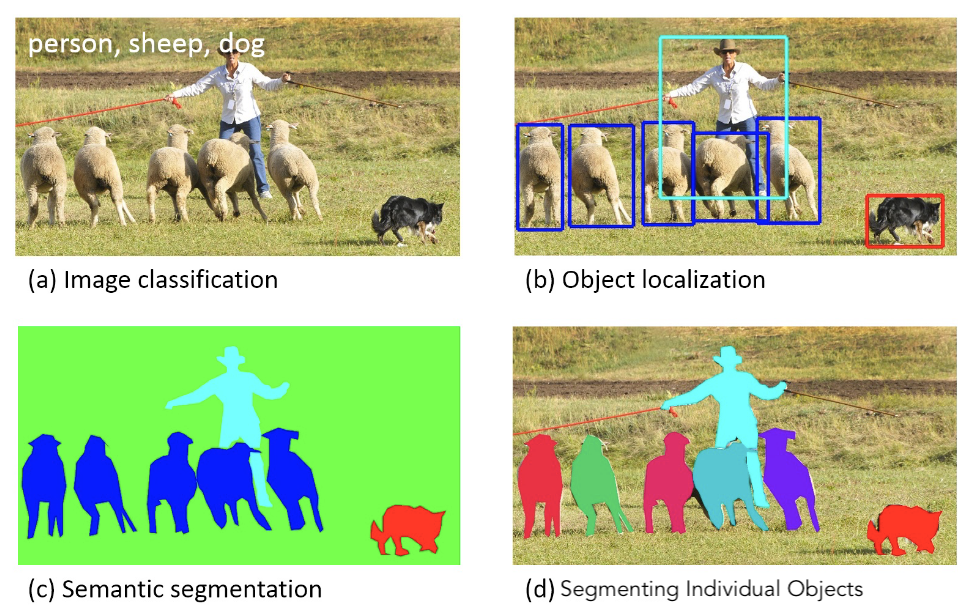
\includegraphics[width=0.6\linewidth]{images/classification_types.png}
    \caption{Types of classification in machine vision. Reproduced from Lin et al. \cite{linMicrosoftCOCOCommon2014}}
    \label{fig:classification_types}
\end{figure}

\begin{figure}[b]
    \centering
    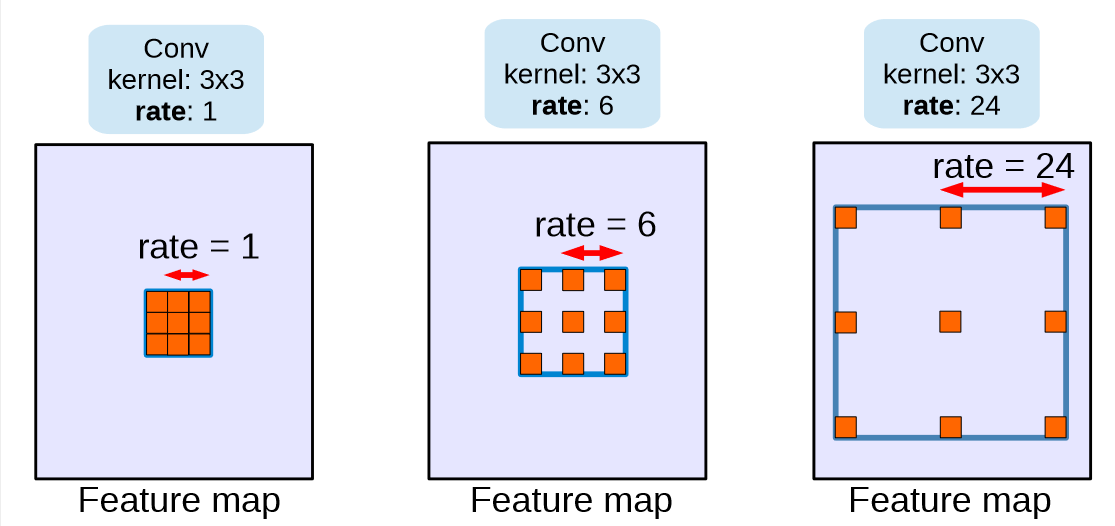
\includegraphics[width=0.6\linewidth]{images/atrous_convolution.png}
    \caption{Atrous convolution with a 3x3 kernel, showing increasing FOV. Reproduced from Chen et al. \cite{chenRethinkingAtrousConvolution2017}}
    \label{fig:atrous_convolution}
\end{figure}

\pagebreak
\subsubsection{Autonomous Driving}
Autonomous driving and autonomous wheelchair control involve similar challenges,
including drivable area segmentation and object detection. As described previously, many machine learning
models utilise an image classification backbone to extract features from an image, with a `detection head'
then used for the final prediction.

Running multiple classification backbones for different models can be inefficient, as
the work of feature extraction is duplicated many times over. One way to improve the performance
of the autonomous system is to share a classification backbone between models, and use different detection
heads for various tasks.

An example of this architecture is HydraNets \cite{karpathyTeslaAIDay2021}, a machine learning model used by
Tesla to perform tasks such as traffic light detection, lane prediction, and object detection efficiently.
Other machine learning models that utilise this architecture include YOLOP \cite{wuYOLOPYouOnly2021} and
Hybridnet \cite{vuHybridNetsEndtoEndPerception2022}, which focus on lane segmentation, drivable area segmentation,
and object detection. The model architecture of YOLOP is shown in \cref{fig:yolop}.

This approach is valuable in situations where compute hardware is limited. Real-time applications such as
autonomous wheelchair control require fast inference times to react to obstacles in the surrounding environment.

\begin{figure}[b]
    \centering
    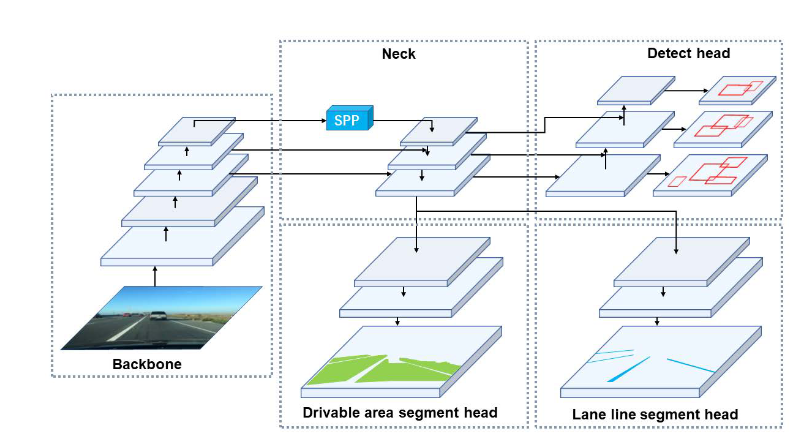
\includegraphics[width=0.65\linewidth]{images/yolop.png}
    \caption{YOLOP model architecture. Reproduced from Wu et al. \cite{wuYOLOPYouOnly2021}}
    \label{fig:yolop}
\end{figure}

To train these ML models, a pre-trained model backbone (on a dataset such as ImageNet \cite{jiadengImageNetLargescaleHierarchical2009})
is retrained on a driving dataset. This technique is known as transfer learning, and can vastly reduce the amount of time required
to train a new model.
Driving datasets such as Cityscapes \cite{cordtsCityscapesDatasetSemantic2016} and Berkeley DeepDrive \cite{yuBDD100KDiverseDriving2018}
can be used for this purpose. Additionally, game-engine based driving simulators such as CARLA \cite{dosovitskiyCARLAOpenUrban2017} can be used to generate a
synthetic dataset for training.

% U-net, deepnet

% classification, localization, segmentation, video, datasets
% SLAM, mapping, hybridnet, etc.
% Transfer Learning & Datasets

\pagebreak
\subsection{Assistive Control}
Once an understanding of the 3D scene has been built, the user can be navigated through the environment.
The surrounding environment is generally represented as an occupancy grid \cite{elfesUsingOccupancyGrids1989},
which is a top-down view of the area where each grid cell indicates the probability that it is occupied
by an obstacle. It is possible to include more detailed information about
paths and obstacles by adding more information to the occupancy grid.

In semi-autonomous control, the user decides the desired speed and direction of the wheelchair, with any intervention only
occurring before a collision takes place. This is in contrast to full autonomy, where the user specifies the
desired end goal and the wheelchair navigates to that goal \cite{wangS2P2SelfSupervisedGoalDirected2021}.
%In full autonomous control, SLAM is required to build a global map of the surroundings - this is not necessary
%for semi-autonomous control, as only a local map is needed for navigation assistance.

\subsubsection{Path-Based Algorithms}
Path-based algorithms take an occupancy grid as an input and output a path between the start point and a goal point.
A* is an example of this and uses a heuristic to efficiently find the shortest path between the start and end point.
Other algorithms such as RRT* (rapidly-exploring random tree) \cite{karamanSamplingbasedAlgorithmsOptimal2011} build a tree from randomly sampled points
to find a path to the goal node. RRT* may not find the shortest path initially, but can find an efficient path with much less
computation required.

\begin{figure}[b]
    \centering
    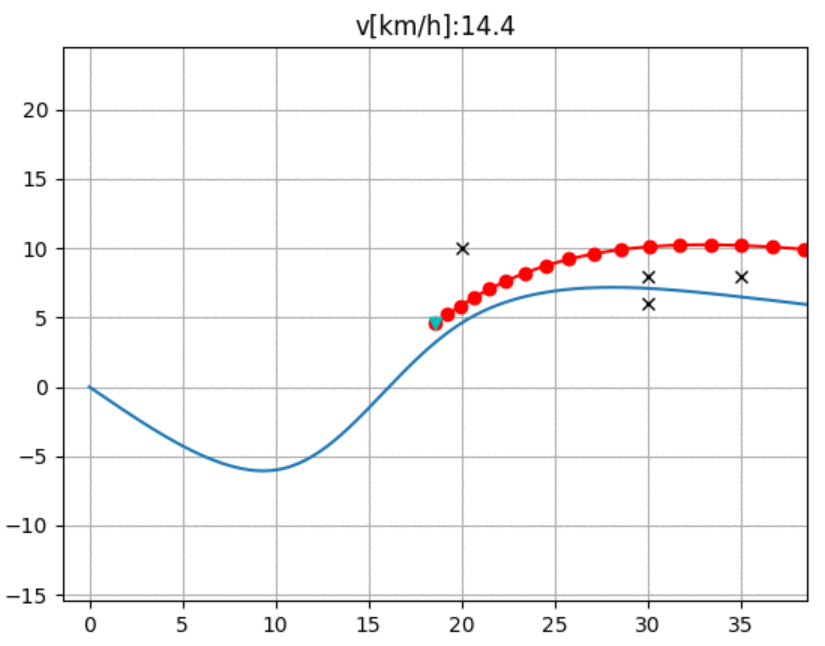
\includegraphics[width=0.5\linewidth]{images/frenet_frame_local_path.png}
    \caption{Fren\'et-Frame path planning, with reference path and local path illustrated. Reproduced from Sakai et al. \cite{sakaiPythonRoboticsPythonCode2018}}
    \label{fig:frenet_frame_local_path}
\end{figure}

One potential issue with these two algorithms is that they fail to take into account the smoothness of the resulting path.
Although the path may be short, sharp changes in the trajectory could be uncomfortable for the user.

Trajectory planning algorithms aim to solve this - one such algorithm is optimal-control in a Fren\'et-Frame \cite{werlingOptimalTrajectoryGeneration2010},
which can be used in autonomous vehicle control.
This algorithm takes a reference path as an input and outputs a local path that avoids collisions and minimises jerk (rate of change of acceleration).
This is done by generating sample trajectories (represented with quintic polynomials), removing those which cause collisions, and choosing
the remaining trajectory with the lowest change in acceleration. \Cref{fig:frenet_frame_local_path} illustrates the reference path, obstacles, and generated
local path in an example scenario.
It should be noted that this algorithm still requires a reference path, which could be generated
with one of the pathfinding algorithms mentioned above.

\subsubsection{Local Algorithms}
Local algorithms only consider obstacles currently in the proximity of the wheelchair,
and use this information to set the current speed and direction of the wheelchair.
VFH+ (vector field histogram) \cite{ulrichVFHReliableObstacle1998} is one example, which
has been applied to wheelchair control algorithms in prior work \cite{tomariEnhancingWheelchairControl2014}.
VFH+ calculates a polar obstacle density histogram around the robot based on the occupancy grid.
The histogram is then binarized, to classify sectors around the robot as either occupied or not occupied.
Next, a masked polar histogram is generated, which excludes paths that are not possible given the robots
turning radius and kinematics. Finally, a safe direction is chosen which is nearest to the user's desired direction.
An example binary histogram is shown in \cref{fig:binary_histogram_vfh}; the chosen direction avoids the obstacle in the
desired direction.

\begin{figure}[b]
    \centering
    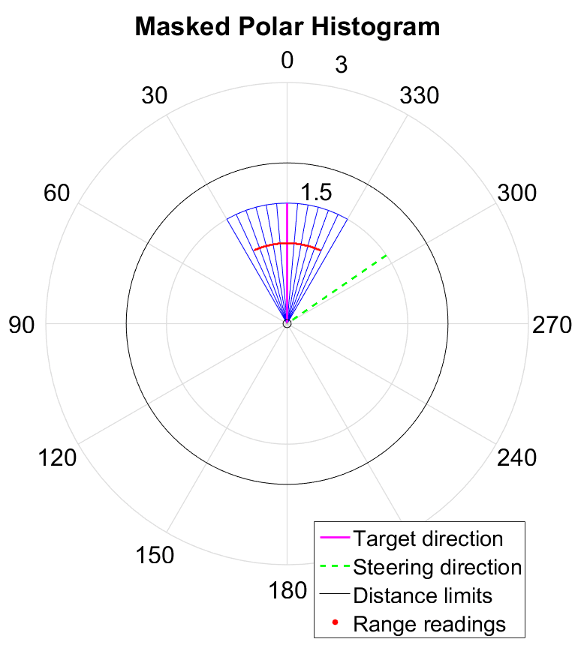
\includegraphics[width=0.38\linewidth]{images/binary_histogram_vfh.png}
    \caption{VFH+ binary histogram, representing the direction of obstacles. Reproduced from MathWorks \cite{mathworksVectorFieldHistogram2022}}
    \label{fig:binary_histogram_vfh}
\end{figure}
\pagebreak
An advantage to this algorithm is that it gives the user more fine-grained control over their speed and direction,
rather than planning a path to their assumed goal.
However an issue with VFH+ is that it does not control the wheelchair's speed, and instead only finds a safe direction.
Ideally, the wheelchair should slow down if an obstacle is present.

Another approach to assistive control with local algorithms is haptic feedback. Rather than
blending inputs from the autonomous software and the user, the joystick itself is actuated
to make it more difficult to move in the direction of obstacles \cite{kondoNavigationGuidanceControl2008}\cite{vanderpoortenPoweredWheelchairNavigation2012}.
An advantage of this approach is that it gives the user total control over which direction of movement they choose,
however, the additional force required to actuate the joystick may fatigue the user.

%\subsubsection{Path and Trajectory Planning}
%Path planning involves finding a path from the current location to the goal location.

%\subsubsection{Feedback and Control Blending}
%Alternative methods which can be used to provide assistance to the user are haptic feedback and control blending.


% Inputs
% Semi-autonomy
% Full autonomy
% Path Planning
% Obstacle avoidance
% 3D - 2D mapping

% Indoor vs Outdoor assistance.
% Sensors
% Machine Learning
%\cite{tomariEnhancingWheelchairControl2014}

\cleardoublepage

\section{METHODOLOGY}
\subsection{Hardware}
The smart wheelchair must sense the environment, process this information,
and maneuver within the environment. Doing so requires hardware, including a
sensor system, compute unit, and motor controller.

The literature review compares several types of sensors and manufacturers for these sensors.
An RGB-D camera was selected for this application, as they provide high-resolution images and depth
information at a commercially viable price point. High-resolution image data builds flexibility into
the system, as popular machine learning algorithms can be utilised.

This RGB-D camera must be mounted to the wheelchair at an appropriate point. The front of the
joystick control unit was selected for the reasons below:
\begin{enumerate}[topsep=0pt,itemsep=-1ex,partopsep=1ex,parsep=1ex]
    \item A clear view of the environment in front of the wheelchair is provided.
    \item The user does not obstruct the camera's view in any wheelchair configuration.
    \item The camera does not obstruct the user's view or comfort in any wheelchair configuration.
    \item When exiting the wheelchair, the user can move the joystick control unit and camera
            out of the way using the existing joystick control unit mount.
\end{enumerate}
Some considerations must be addressed when using this mounting point.
\begin{enumerate}[topsep=0pt,itemsep=-1ex,partopsep=1ex,parsep=1ex]
    \item Unstable video footage could be observed due to low rigidity in the joystick control unit mount.
    \item Mount point is \SI{790}{\milli\metre} forward from the back of the wheelchair, impacting
            the visibility of the rear and side of the wheelchair.
    \item Doorway maneuverability is impacted if RGB-D camera width exceeds \SI{150}{\milli\metre}.
\end{enumerate}
This sensor mounting point is positioned on the right-hand side of the wheelchair,
\SI{720}{\milli\metre} above the ground and \SI{300}{\milli\metre} behind the
front of the wheelchair (measured from the footplate), and can be seen in \cref{fig:wheelchair_zed_1}.

The RGB-D camera model selected was the Stereolabs ZED Mini, which uses passive stereo-vision
to generate a depth map. Active IR RGB-D cameras were not viable for this application
due to their poor outdoor performance and range. The width of the ZED Mini also fulfils the
size requirements of the selected mounting point.

Smart wheelchair applications such as wheelchair docking require
obstacle detection on all sides of the wheelchair. To satisfy this requirement, a
Cygbot CygLiDAR D1 was procured for short-range detection of obstacles at the rear of the
wheelchair. Nicolas Lee, a project student focused on
wheelchair navigation to personal vehicles, selected this sensor. It should be noted that
this sensor was not used for navigation assistance as part of this thesis.

% Sensor mount design
A 3D printed sensor mount was designed to fix the ZED Mini to the wheelchair mounting point.
This sensor mount was based on a ZED Mini mount designed by Walter Lucetti at Stereolabs \cite{lucettiStereolabsZEDMini2018},
with several major modifications made using Autodesk Inventor:
\begin{enumerate}[topsep=0pt,itemsep=-1ex,partopsep=1ex,parsep=1ex]
    \item Width of the mount was greatly reduced to improve maneuverability.
    \item A mounting plate was added, allowing the sensor mount to bolt onto
            the existing joystick control unit.
    \item Some sensor clips were modified to make sensor removal more convenient.
    \item Sharp corners were rounded to reduce the risk of injury to a user.
\end{enumerate}
\Cref{fig:zed_mount} shows a render of the ZED Mini camera and custom mount.
\Cref{fig:wheelchair_zed_1} shows the ZED Mini camera mounted to the joystick control unit
on the wheelchair.

\begin{figure}[b]
    \centering
    \begin{minipage}[b]{.4\textwidth}
      \centering
      \captionsetup{width=.8\textwidth}
      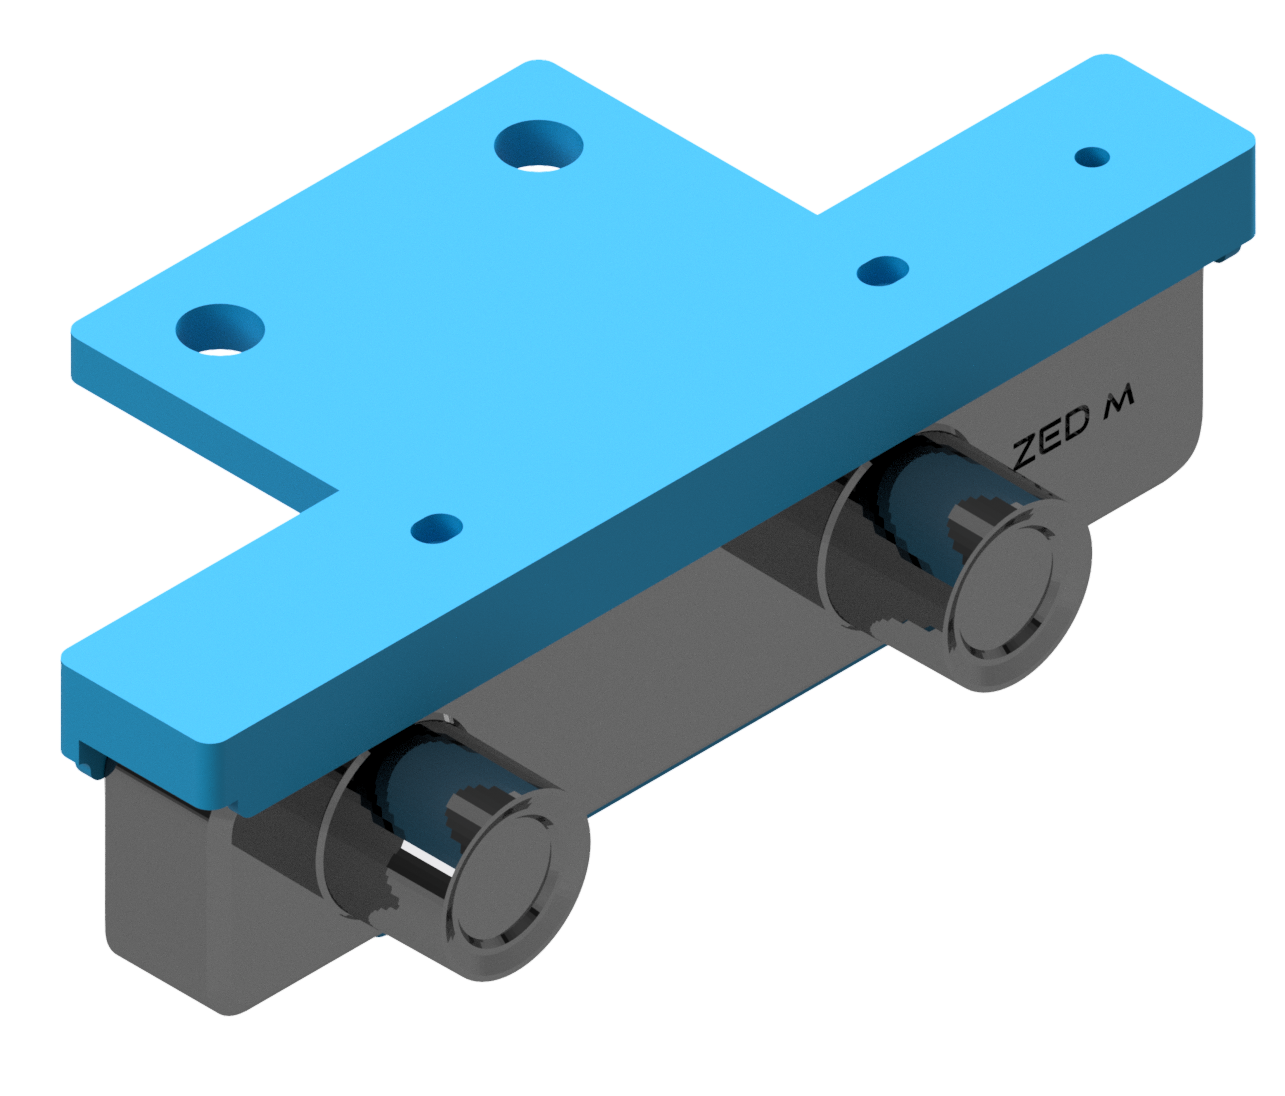
\includegraphics[width=\linewidth]{images/zed_mount.png}
        \captionof{figure}{3D render of ZED Mini camera and wheelchair mount}
        \label{fig:zed_mount}
    \end{minipage}%
    \begin{minipage}[b]{.48\textwidth}
        \centering
        \captionsetup{width=.8\textwidth}
        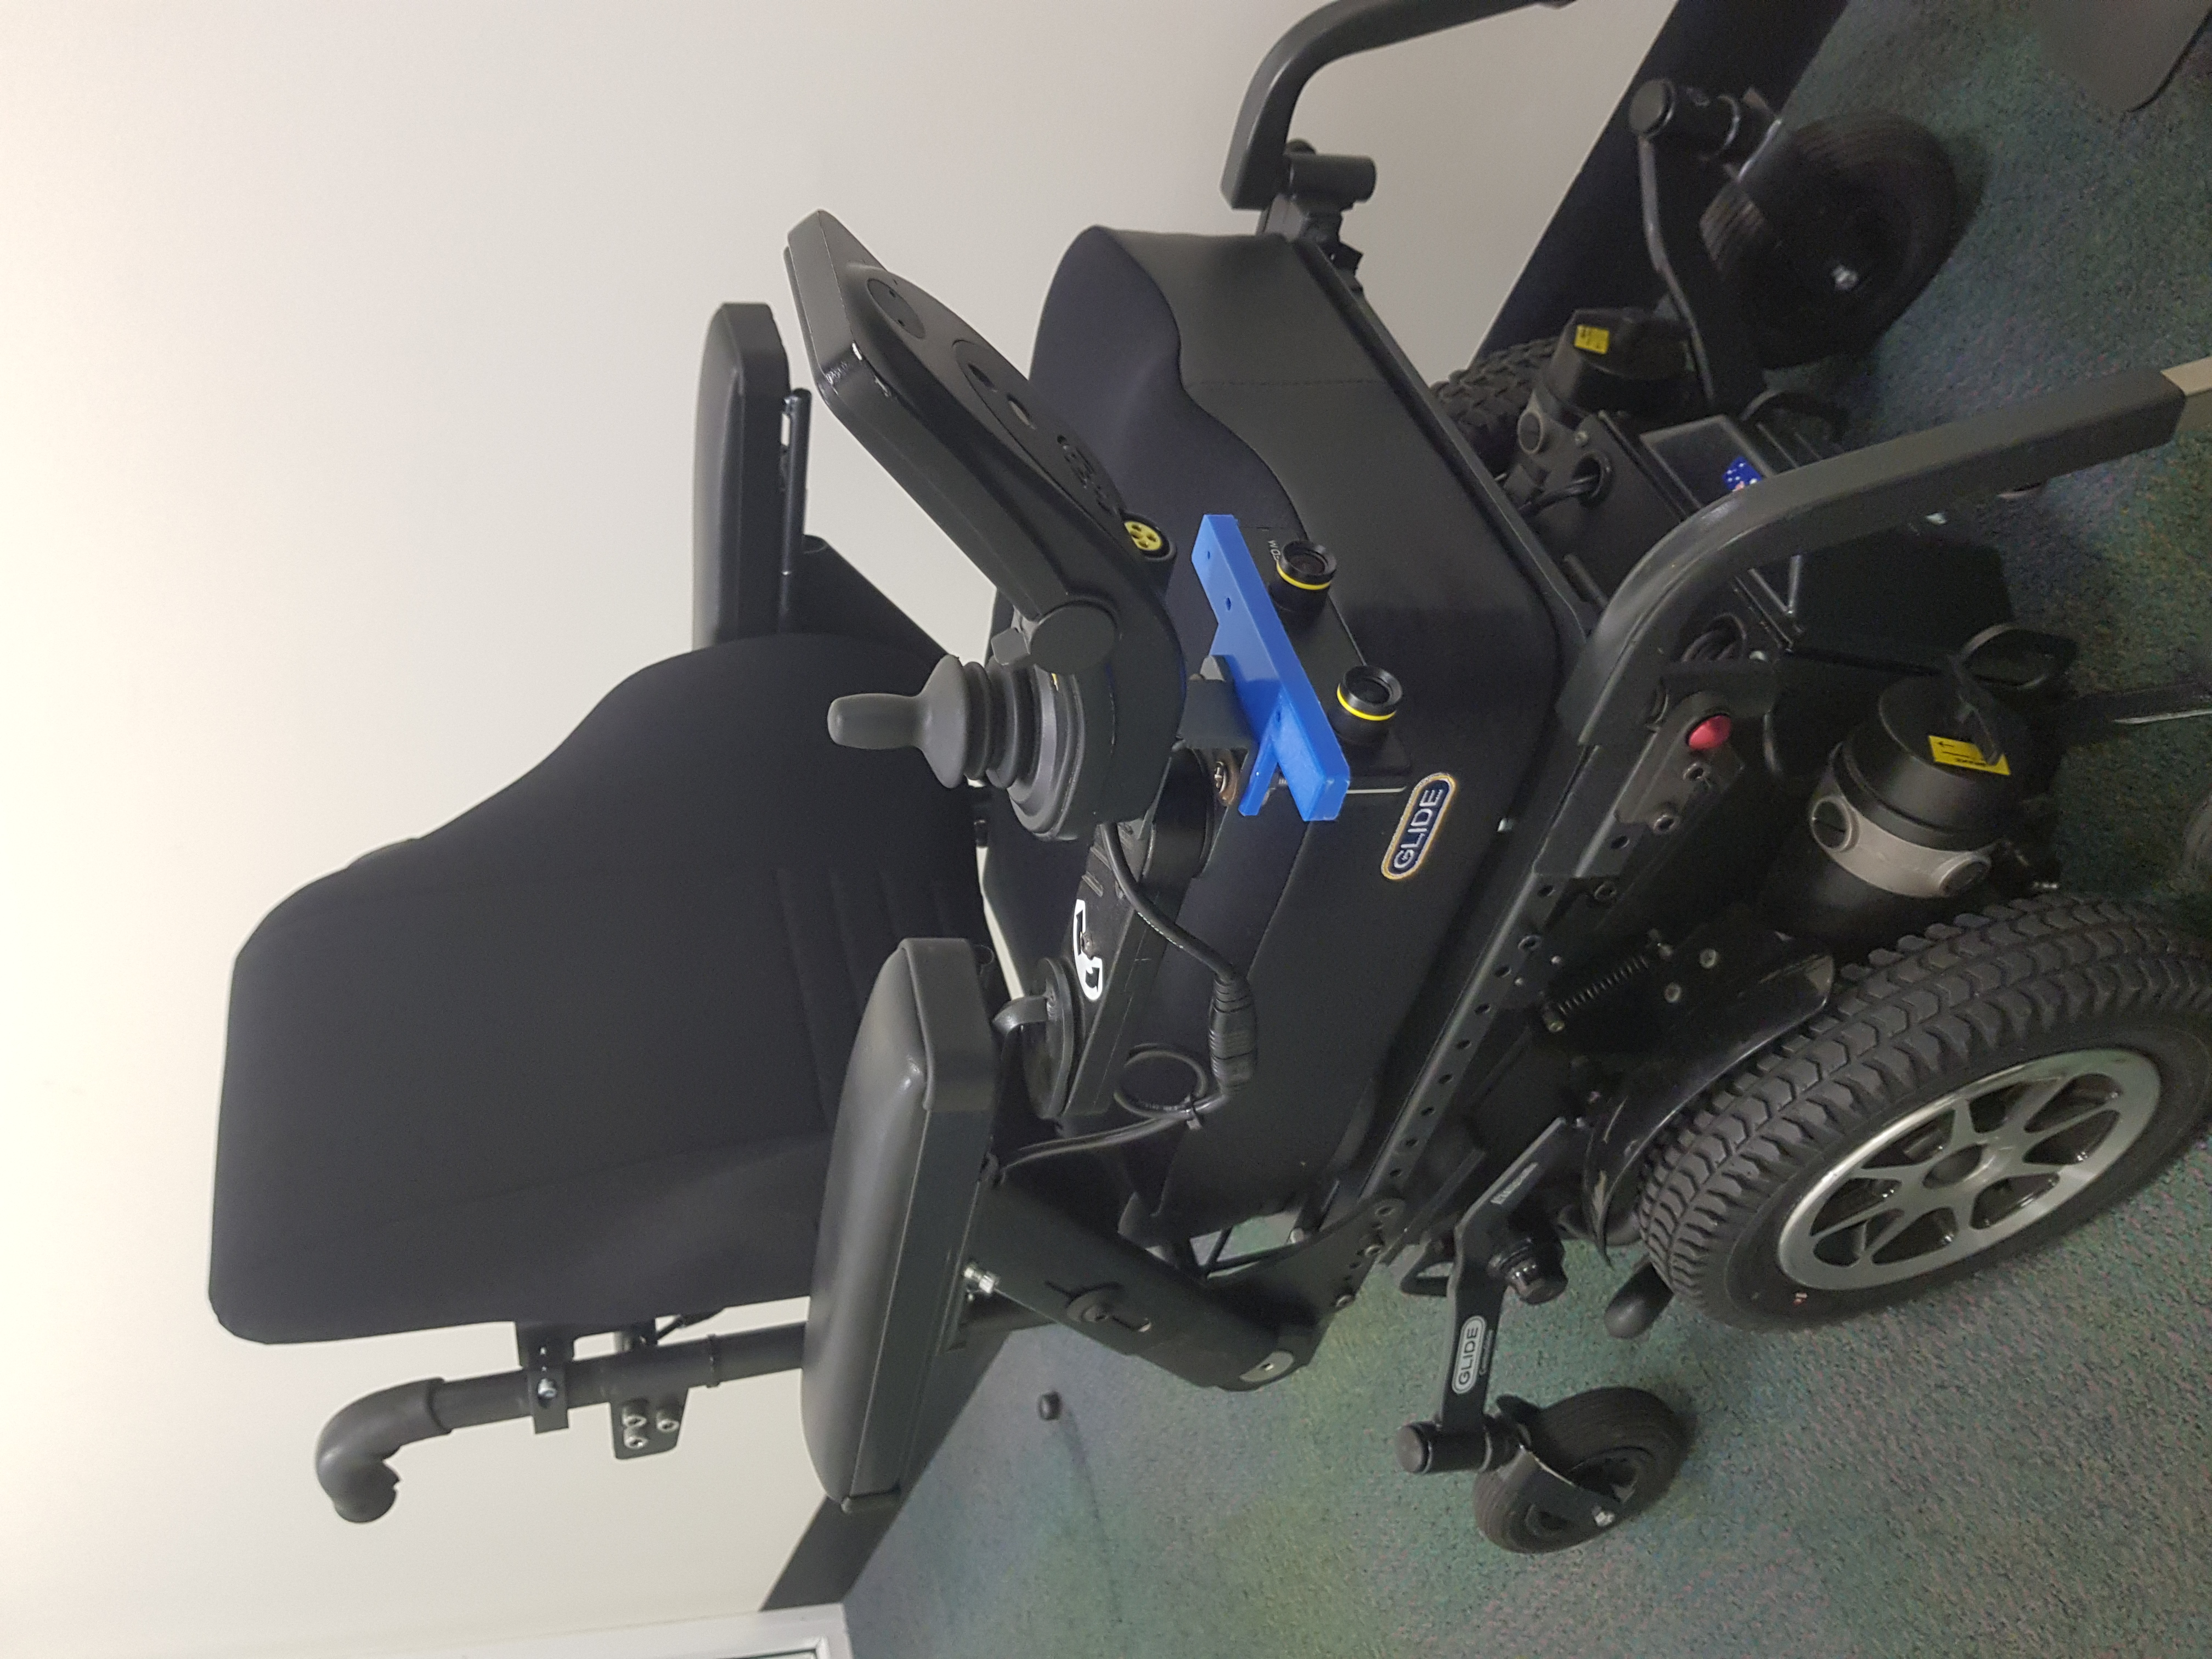
\includegraphics[height=\linewidth,angle=270,origin=c]{images/wheelchair_zed_1.jpg}
        \captionof{figure}{ZED Mini camera and mount fixed to joystick control unit}
        \label{fig:wheelchair_zed_1}
    \end{minipage}
\end{figure}

In addition to the RGB-D camera and Lidar sensor, an AI accelerator is required to process the sensors'
output and run ML algorithms. The literature review compares several AI accelerators across categories
such as computational speed, power draw, and price. An Nvidia Jetson Xavier NX was selected for this task,
as the Stereolabs ZED Mini requires a CUDA-enabled accelerator to generate a depth map. This accelerator's
low power draw and small form factor are suited for mobile robot applications such as smart wheelchairs.
Due to budget constraints and the ongoing chip shortage, the project team could not procure this AI accelerator.
Instead, a laptop with an RTX 3080 graphics card was used to record datasets and evaluate the speed of
ML algorithms.

A CentroGlide powered wheelchair was used as a base for the smart wheelchair functionality.
The CentroGlide is a mid-wheel drive wheelchair with two independently controlled powered wheels and four
unpowered castor wheels.
A joystick module communicates user commands to a power module, which controls
each motor. An intelligent seating module (ISM) adjusts the seat tilt and recline \cite{glideCentroGlideOWNERUSER2022}.
This wheelchair is \SI{1100}{\milli\metre} in length (including footplate), \SI{620}{\milli\metre}
in width, and \SI{1030}{\milli\metre} in height.
Communication between the joystick module, power module, and ISM is shown in \cref{fig:module_communication}.

\begin{figure}[b]
    \centering
    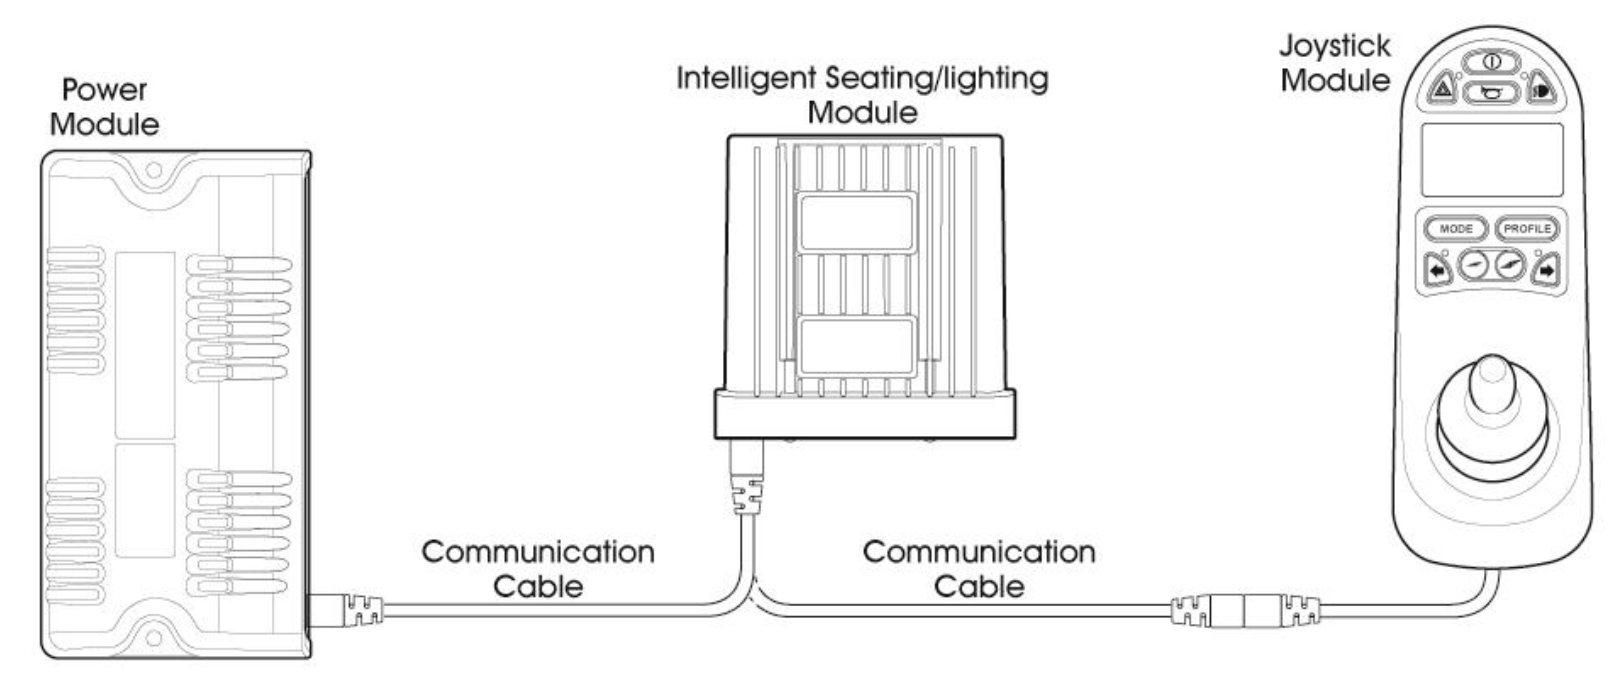
\includegraphics[width=0.7\linewidth]{images/module_communication.png}
    \caption{Communication between CentroGlide control modules. Reproduced from Curtiss-Wright. \cite{curtiss-wrightPGDRIVESTECHNOLOGY2016}}
    \label{fig:module_communication}
\end{figure}

An input controller is being developed by project student Brian Smith to intercept
commands from the joystick module and communicate with the smart wheelchair navigation system.
The input controller enables the navigation system to receive user commands and choose a safe
direction and speed for the wheelchair.
A high-level protocol between the navigation system and input controller has been designed
and is detailed in the future work section of this thesis. The input controller will validate the
navigation system's output, ensuring that the user
can still safely maneuver the wheelchair in the case of a software failure.
Additionally, a motor controller was developed by project student
Kosma Egan, which receives commands from the input controller to drive and monitor the motors.
\pagebreak

\subsection{Dataset Collection}
An RGB-D wheelchair driving dataset was collected around Curtin university
to test and evaluate the performance of the navigation assistance system.
This dataset is \SI{7.14}{\giga\byte} in size and \SI{47}{\minute} in length
and includes features such as indoor and outdoor navigation, doorways, pedestrians,
elevator use, wheelchair access ramps, and car parks. A link to the dataset
can be found in Appendix C.

This dataset was collected using the ZED Mini and is encoded in the proprietary Stereolabs SVO file format, which can be read using the ZED SDK.
This format includes image data from left and right cameras, IMU data, and metadata such as
timestamps. Depth map and point cloud data are not stored in the dataset and are instead generated when
the file is read using the ZED SDK.

Four compression modes are available during dataset collection: Lossless (PNG), Lossy (JPG), H.264 (Video),
and H.265. Both video compression modes require a CUDA-enabled device during dataset collection.
A 10-second sample dataset was recorded for each compression mode to evaluate image quality and
file size (results in \cref{table:dataset_compression_modes}). Due to the smaller file size, H.264 compression was used when collecting the wheelchair driving dataset.
\Cref{fig:zed_sample_dataset} shows an example image frame and depth map from the dataset.

\begin{table}[H]
    \centering
    \begin{adjustbox}{width=0.7\textwidth}
    \begin{tabular}{c c c c}
    \toprule
    Compression mode & File size & Relative increase & Image quality \\
    \midrule
    Lossless (PNG) & \SI{1240}{\mega\byte} & 41 & Ok \\
    Lossy (JPG) & \SI{640}{\mega\byte} & 21 & Some interlacing \\
    H.264 & \SI{30}{\mega\byte} & 1 & OK \\
    H.265 & \SI{30}{\mega\byte} & 1 & Some frame tearing \\
    \bottomrule
    \end{tabular}
    \end{adjustbox}
    \caption{Comparison between dataset compression modes}
    \label{table:dataset_compression_modes}
\end{table}

\begin{figure}[H]
    \centering
    \begin{subfigure}{.48\textwidth}
        \centering
        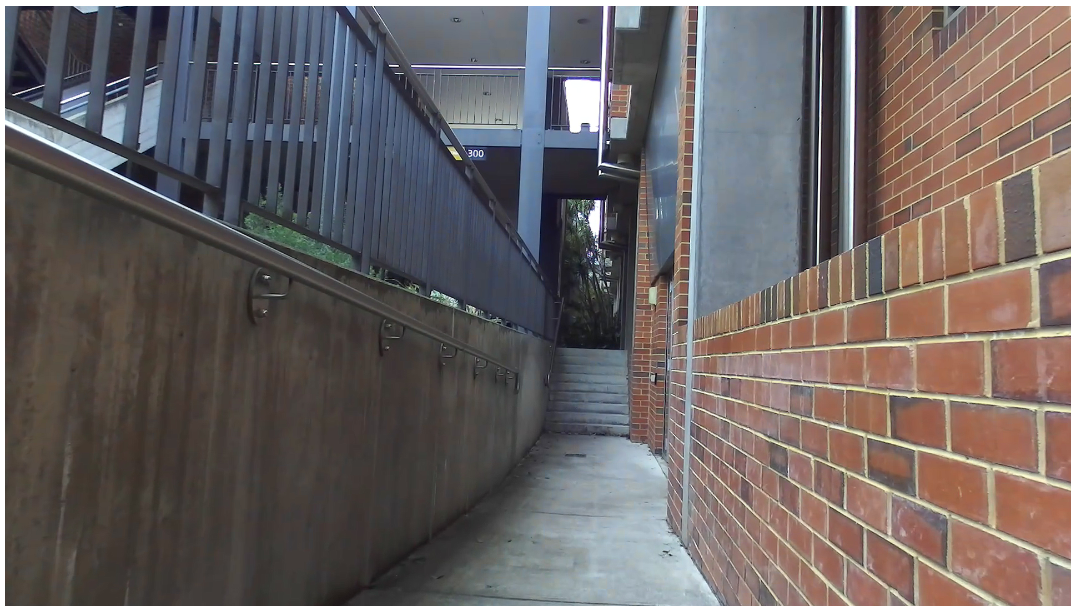
\includegraphics[width=\linewidth]{images/zed_sample_image.png}
        \caption{Image frame}
    \end{subfigure}
    \quad
    \begin{subfigure}{.47\textwidth}
        \centering
        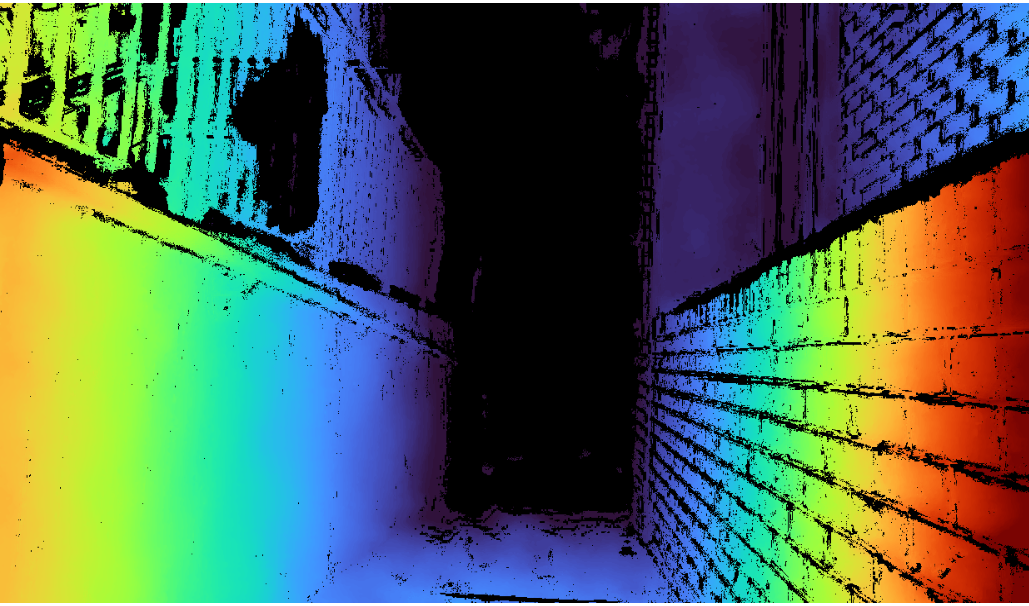
\includegraphics[width=\linewidth]{images/zed_sample_depth.png}
        \caption{Depth map}
    \end{subfigure}
    \caption{Sample data from the Curtin university RGB-D wheelchair driving dataset}
    \label{fig:zed_sample_dataset}
\end{figure}
\pagebreak

After some analysis of the raw point cloud data from the Curtin RGB-D driving dataset,
it was found that the camera was slightly tilted upwards while recording the dataset.
This angle was mostly constant between data collection periods
and was likely due to the ergonomics and tilt of the joystick control unit.
An example of this tilt can be seen in \cref{fig:meshlab_point_cloud}; note
that the floor is angled downwards due to the tilt of the RGB-D camera.
Meshlab was used to determine the coordinates of points
on the ground at a close distance and far distance, and calculate the gradient.
This was done for two different point clouds, one indoor and one outdoor.

\begin{figure}[b]
    \centering
    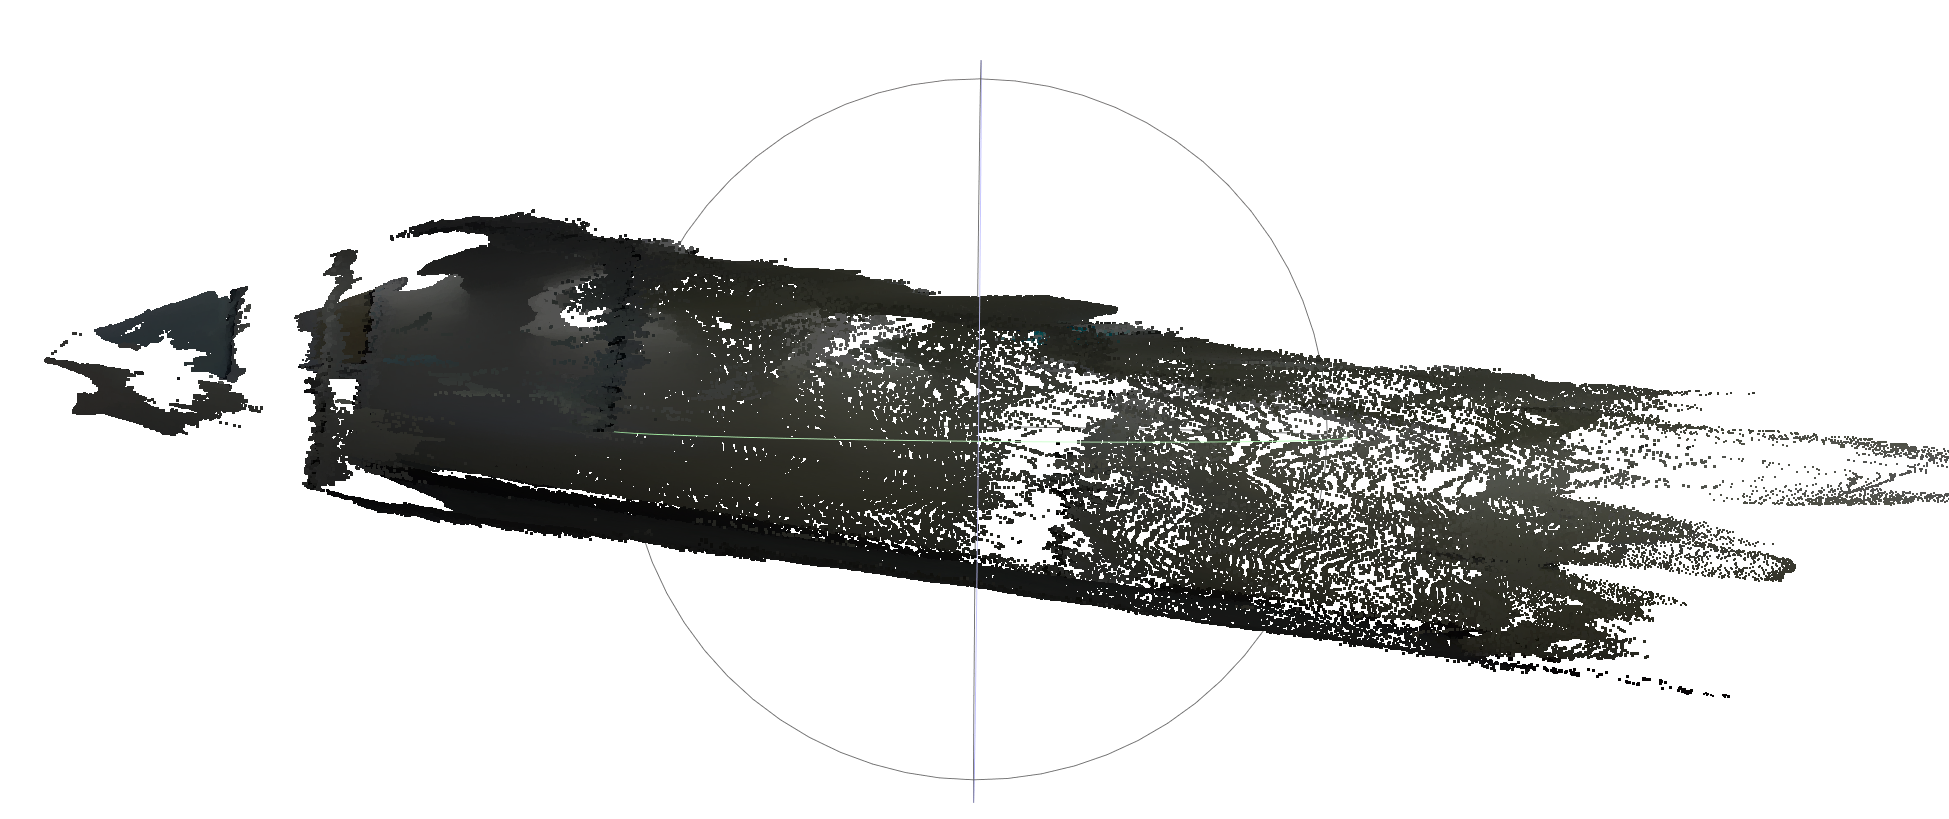
\includegraphics[width=0.8\linewidth]{images/meshlab_point_cloud.png}
    \caption{Point cloud information of indoor hallway (visualized with Meshlab). Note the angle of the floor due to sensor tilt}
    \label{fig:meshlab_point_cloud}
\end{figure}

In addition to the RGB-D dataset, a preliminary wheelchair driving video-only dataset was collected around
Curtin university.
This dataset was \SI{34}{\minute} in length and \SI{7.08}{\giga\byte} in size (1920x1080 @ 24 fps)
and collected using a GoPro Hero 4; the experimental setup used to collect this
dataset can be seen in \cref{fig:gopro_dataset_collection}.
This dataset was used to evaluate machine learning scene recognition algorithms
before the ZED Mini had been ordered.

%\vspace{4.0cm}


\subsection{Software}
The software system involves several scene recognition algorithms to update an internal
map of the surrounding area, keeping track of suitable driving paths and static obstacles
such as walls and stairs. Once this map is created, an algorithm blends the
user's input with this information to determine a safe path forward.
Appendix C contains a link to the source code. A block diagram of the software system
and how it interacts with the hardware is shown in \cref{fig:block_diagram}.

\subsubsection{Evaluation of ML models on preliminary dataset}
The preliminary video-only driving dataset was used to evaluate
several machine learning models before the ZED Mini had been ordered.
Object detection models such as YOLOv5 \cite{ultralyticsYOLOv5} and image segmentation models such as
DeepLabv3 \cite{chenRethinkingAtrousConvolution2017} were evaluated for speed, accuracy, and efficacy.
Hybridnets \cite{vuHybridNetsEndtoEndPerception2022}, a machine learning model which
performs drivable area segmentation and object detection on the same backbone, was also evaluated on
this dataset.

To evaluate these models, a video encoder and decoder needed to be created
to feed image frames into the model. This was implemented using a python generator
so that frames in the video could be iterated over within a for loop and only decoded
when required. OpenCV \cite{bradskiOpenCVLibrary2000} was the underlying library used
to decode each video frame into a BGR pixel array.

Some scene processing algorithms do not run in real-time due to hardware limitations or performance issues.
When this occurs, some frames must be dropped during model evaluation to keep the scene model up to date and minimise latency.
The number of frames to drop can be calculated using \cref{eq:frames_to_drop},
where $t_{frame}$ is the time taken to process the previous frame.
A frame is dropped by simply discarding it once decoded.

\begin{equation}
n_{drop} = \ceil{fps\times t_{frame}} - 1
\label{eq:frames_to_drop}
\end{equation}

%First, the ZED SDK is used to communicate with the ZED Mini camera and retrieve image data,
%point cloud data, and depth map data. Next, several scene recognition algorithms
%identify drivable areas and environmental obstacles. A block diagram of the software system
%and how it interacts with the hardware is shown in \cref{fig:block_diagram}.

\begin{figure}[H]
    \centering
    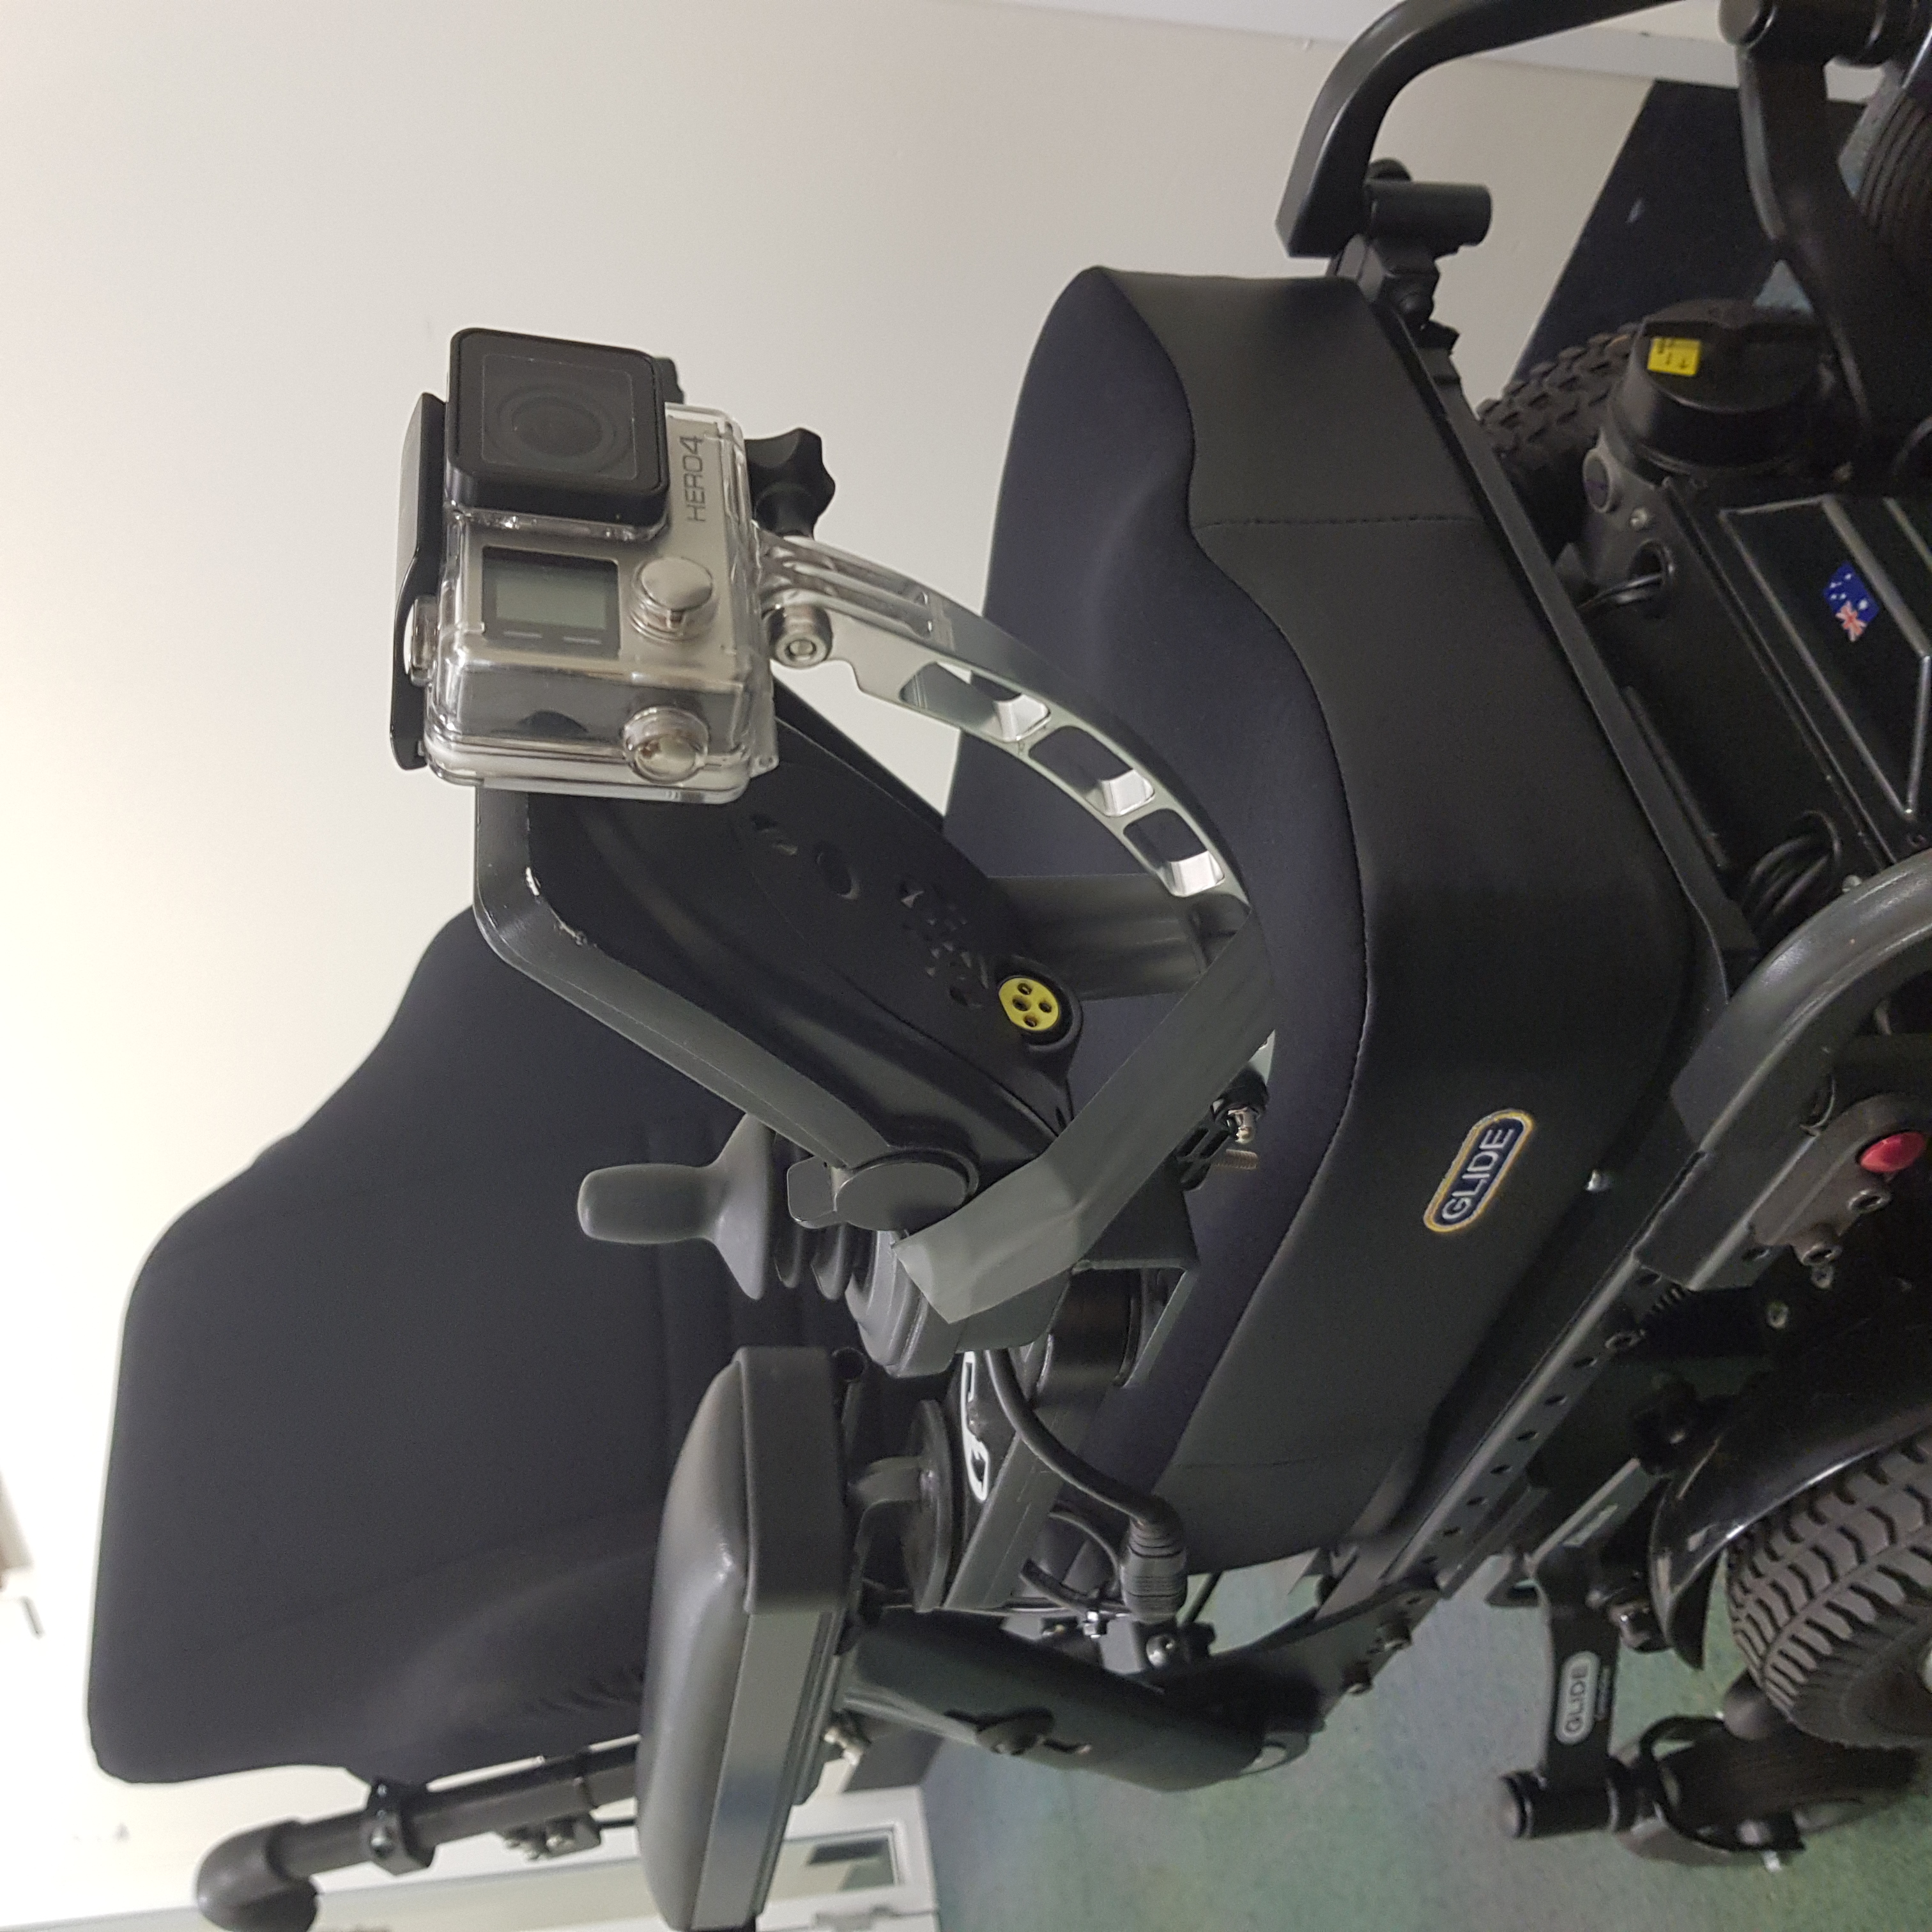
\includegraphics[width=0.45\linewidth,angle=270,origin=c]{images/gopro_dataset_collection.jpg}
    \caption{Experimental setup for preliminary dataset collection}
    \label{fig:gopro_dataset_collection}
\end{figure}

\begin{figure}[b]
    \centering
    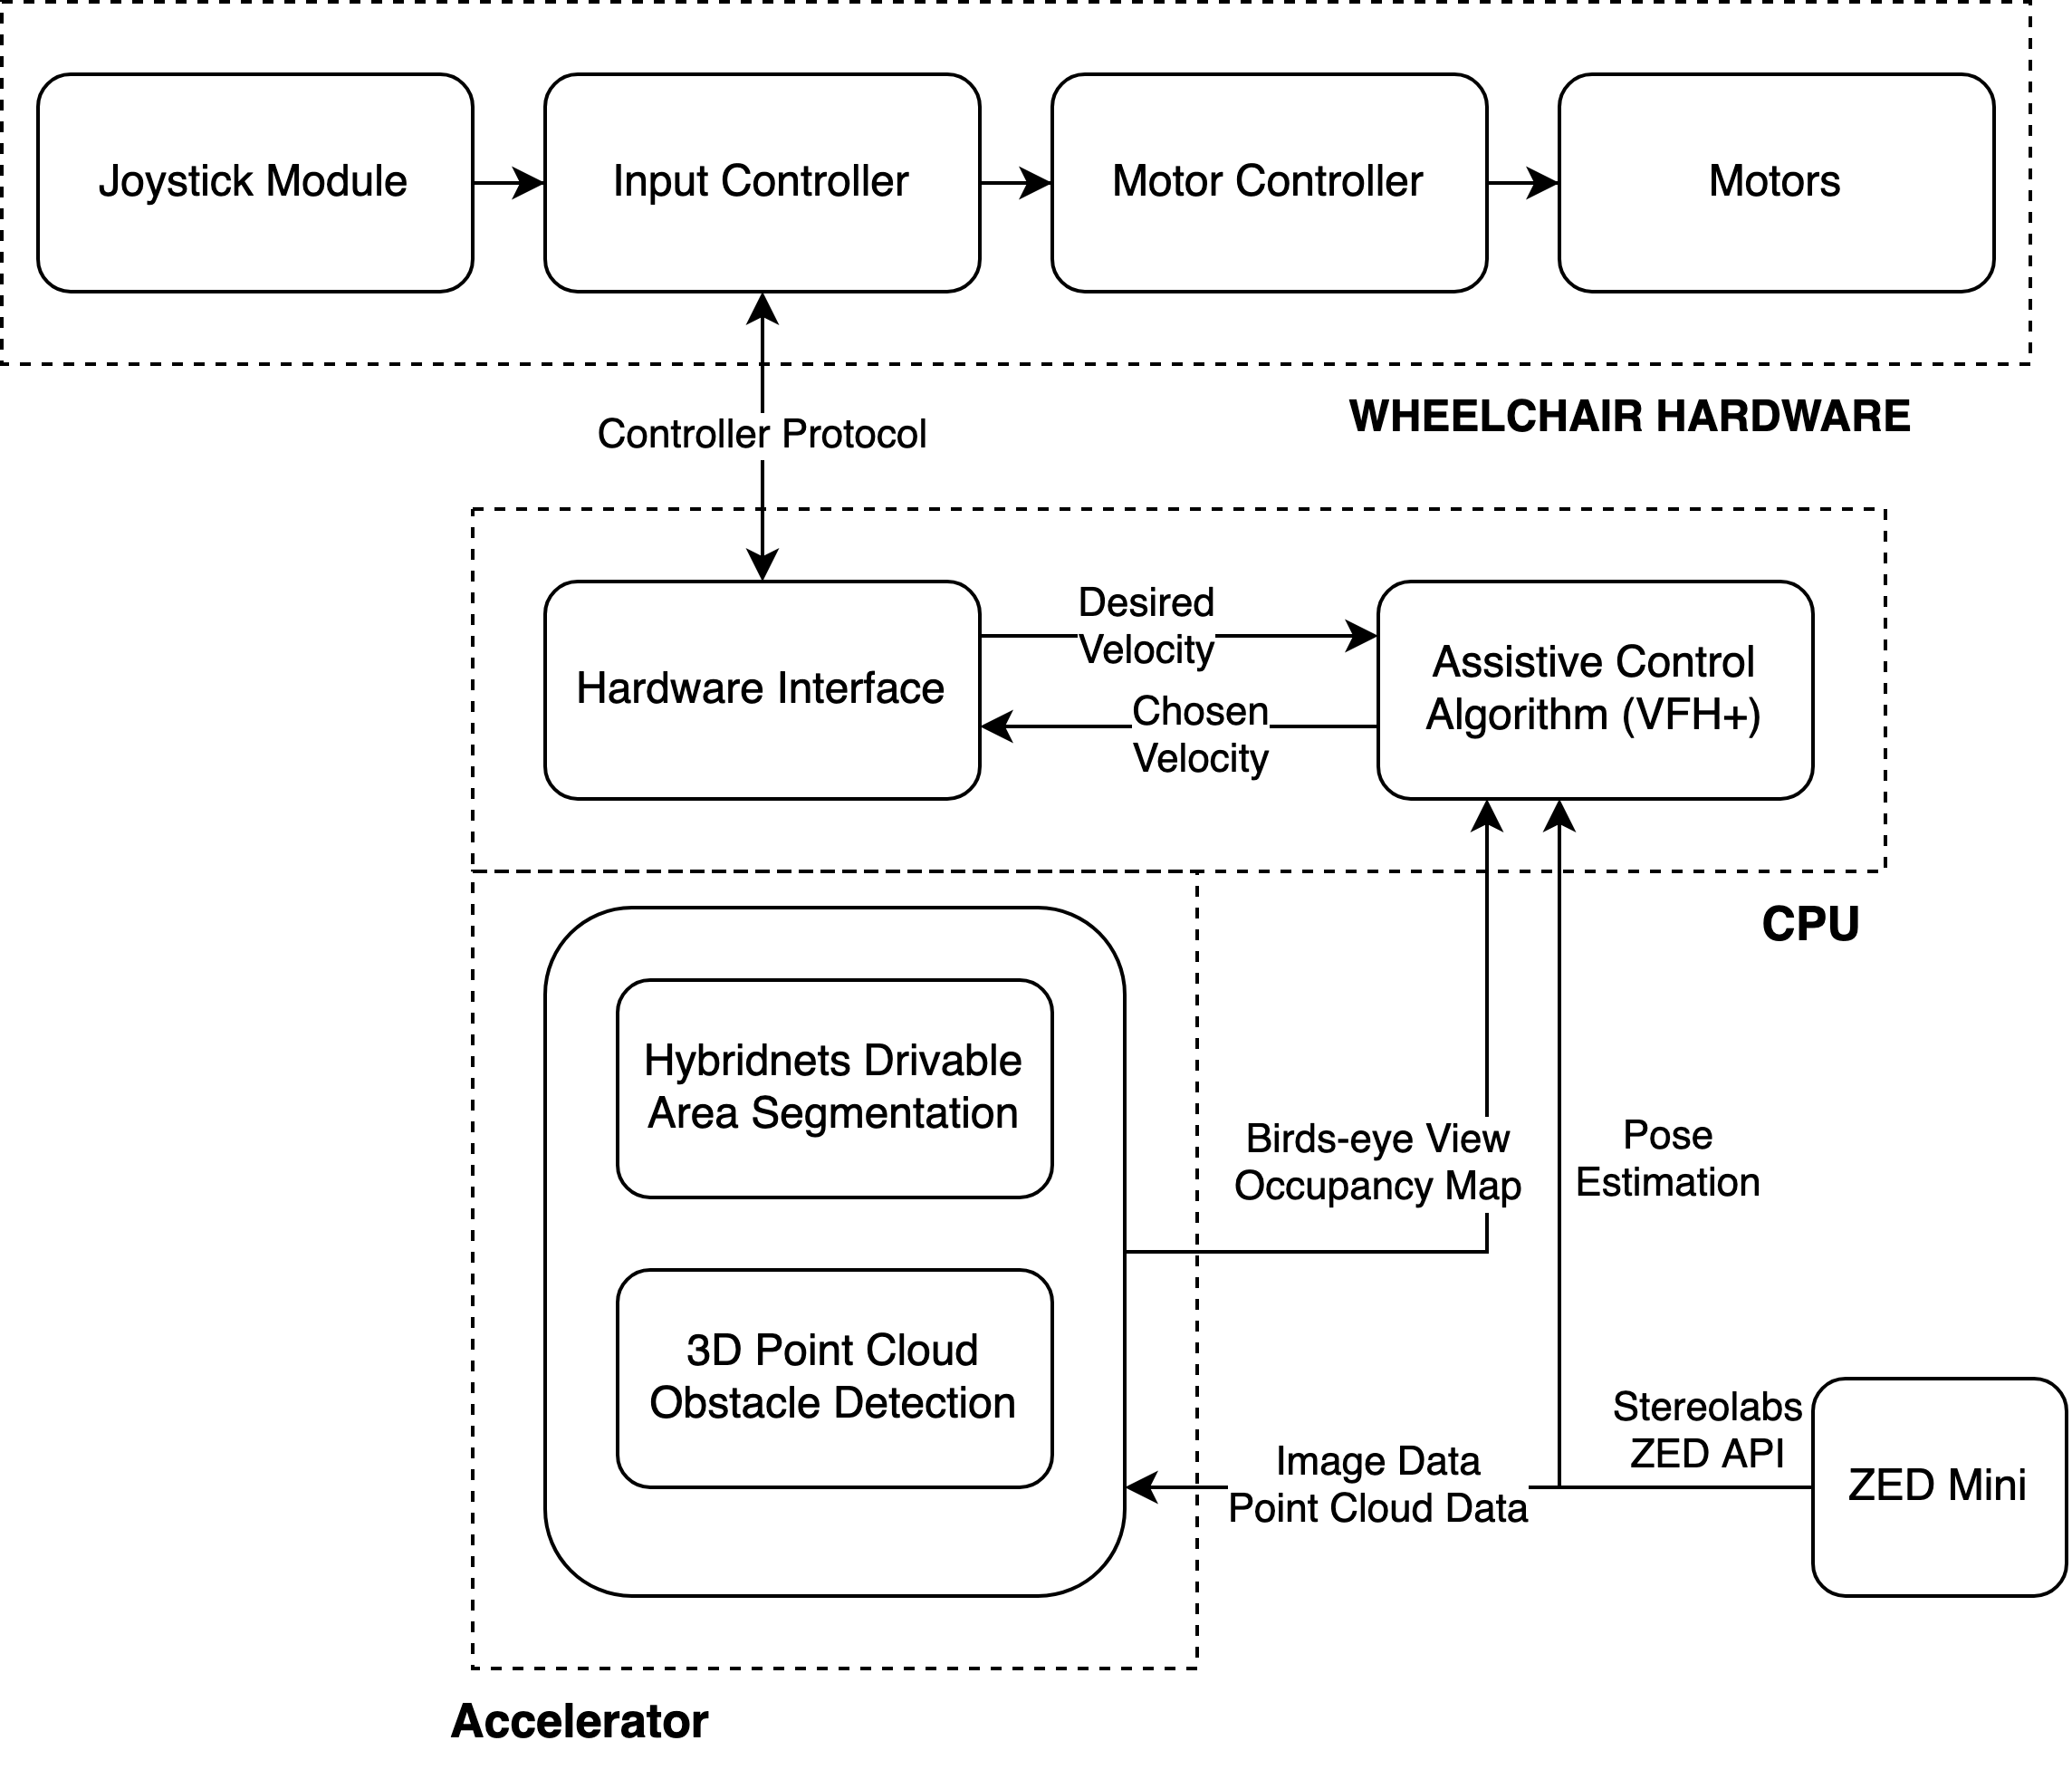
\includegraphics[width=0.8\linewidth]{images/block_diagram.png}
    \caption{Block diagram of software system and interaction with hardware components}
    \label{fig:block_diagram}
\end{figure}
\pagebreak

To avoid training each model from scratch, a pre-trained model is loaded from PyTorch Hub.
The DeepLabv3 and YOLOv5 models were both trained on the MS COCO \cite{linMicrosoftCOCOCommon2014} dataset,
while the Hybridnets model was trained on the Berkeley DeepDrive dataset \cite{yuBDD100KDiverseDriving2018} (BDD100K).

As mentioned in the literature review, some machine learning algorithms can accept
different image classifiers as a model backbone.
MobileNetV3 \cite{howardSearchingMobileNetV32019} was used as a backbone for DeepLabv3 due to its fast performance.
YOLOv5 has 5 model backbones to choose between (nano, small, medium, large, extra-large),
with smaller models sacrificing accuracy for speed. Due to the low latency requirements
of a fast-moving wheelchair, YOLOv5 was evaluated using the small model size (known as YOLOv5s).
Machine learning was done using PyTorch \cite{paszkePyTorchImperativeStyle2019}, due to good compatibility
with existing machine learning models.

\subsubsection{Hybridnets drivable area segmentation}
To improve the performance of the Hybridnets model when segmenting drivable areas,
the performance of the model was quantitatively evaluated using the BDD100K dataset
and the Cityscapes dataset \cite{cordtsCityscapesDatasetSemantic2016}.
The Hybridnets model was also retrained using the Cityscapes dataset
to improve its performance in some scenarios. %% which scenarios?? TODO

%% Training methodology will likely take a while to write.
%This model was used to identify
%which areas were suitable for the wheelchair user to drive on,
%and as a proof of concept for a shared-backbone model architecture.

\subsubsection{Birds-eye view occupancy map}
%The 3D point cloud data was used to identify the corresponding location of a drivable segmented pixel in 3D space.
%This data was used to build a birds-eye view occupancy map of the local area, extending \SI{15}{\metre}
%in front of the wheelchair and \SI{5}{\metre} on either side.
%Large numerical computations were done using Numpy due to efficiency and ease of use.

The output of the Hybridnets drivable area segmentation model is a
segmentation mask, an array that indicates which pixels are drivable
and which are not.
This output must be transformed into a 2D birds-eye view occupancy map,
which indicates the drivable area around the wheelchair. The occupancy
map extends \SI{15}{\metre} in front of the wheelchair and \SI{5}{\metre} on either side.
This occupancy map is a simplified representation of the surrounding world
and is used as an input to the wheelchair control algorithms.

The ZED Mini 3D point cloud data was used
to transform the segmentation mask into an occupancy grid.
The ZED SDK uses the pinhole camera model, as seen in \cref{fig:pinhole_camera_model},
to describe the relationship between pixels on the image plane
and the coordinates of corresponding objects.
The point cloud data is represented as an array the same size as
the original image, with each pixel containing XYZ data about the location of that object
in 3D space.
% add representation diagram
\begin{figure}[b]
    \centering
    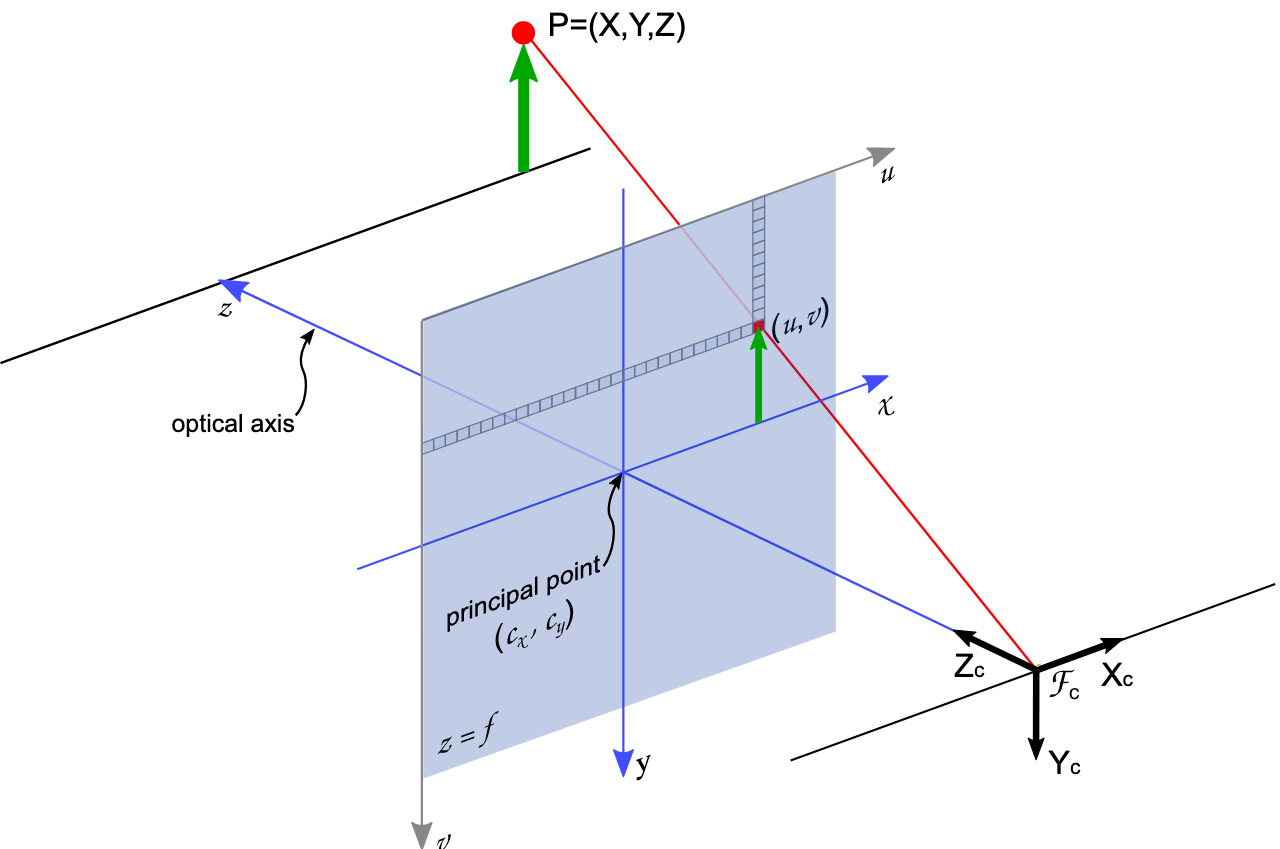
\includegraphics[width=0.6\linewidth]{images/pinhole_camera_model.png}
    \caption{Pinhole camera model. Reproduced from Nvidia \cite{nvidiaVisionProgrammingInterface}}
    \label{fig:pinhole_camera_model}
\end{figure}

To obtain the occupancy map, the point cloud is first filtered using the segmentation mask so that
non-drivable points are removed. The ZED SDK is unable to resolve the depth of some pixels
and instead represents their location as \texttt{nan}; these points are also removed.
Next, the array is simplified by removing non-essential information such as colour and altitude
data. What remains is an array of XZ points that represent drivable areas
identified by the segmentation algorithm. These XZ points are referenced
using a right-handed y-up coordinate frame, with the origin at the left lens of the ZED Mini;
see \cref{fig:zed_mini_coordinate_frame}.
\begin{figure}[b]
    \centering
    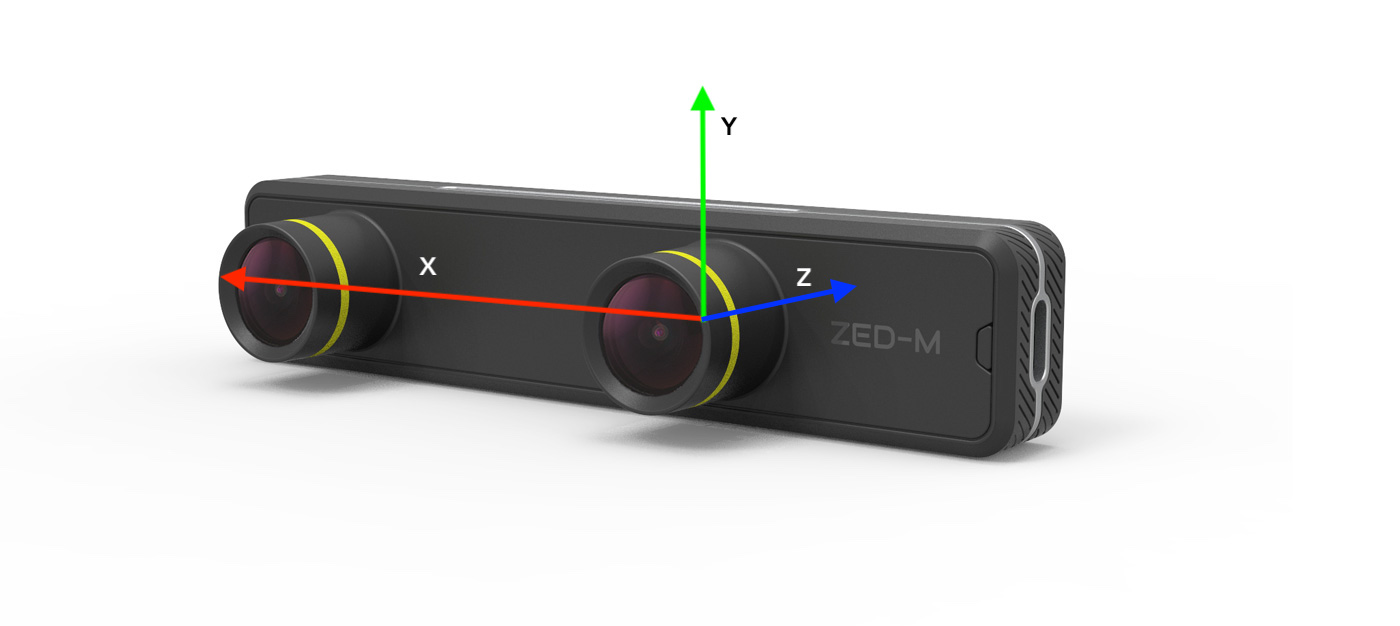
\includegraphics[width=0.9\linewidth]{images/zed_mini_coordinate_frame.jpg}
    \caption{ZED Mini coordinate frame (right-handed y-up)}
    \label{fig:zed_mini_coordinate_frame}
\end{figure}
% Add frame of reference

These points must be scaled to place them on the occupancy grid. This occupancy grid
extends \SI{15}{\metre} in front of the wheelchair and \SI{5}{\metre} on either side,
with each cell of the grid corresponding to a $\SI{25}{\milli\metre}\times \SI{25}{\milli\metre}$ area.
\Cref{eq:occupancy_scaling} was used to scale these points. Note that $p_x$ and $p_z$ are
represented in metres.
\begin{align}
i_x = min\left(max\left(\frac{p_x + 5.0}{0.025}, 1\right), \frac{10.0}{0.025}\right) - 1\\
i_y = min\left(max\left(\frac{p_z + 15.0}{0.025}, 1\right), \frac{15.0}{0.025}\right) - 1
\label{eq:occupancy_scaling}
\end{align}

An issue with the occupancy grid at this stage is that it is rather sparse
due to the one-to-one mapping between segmented pixels and grid cells.
Morphological image processing techniques were used to improve the density of the occupancy map.
The OpenCV \cite{bradskiOpenCVLibrary2000} implementation of morphological dilation was used to
join the space between drivable pixels, to create a continuous driving surface in the occupancy map
rather than many separate pixels. A $10\times 10$ kernel was used to perform this dilation.

\subsubsection{3D point cloud obstacle detection}
Another method that was tested to identify environmental obstacles and drivable areas
was the direct processing of the 3D point cloud data, which removes any use of RGB image data.
One approach that was tested was the inbuilt ZED SDK function \texttt{find\_floor\_plane}.
This function takes the current floor height and camera orientation as arguments
and uses them to identify the floor plane. The \texttt{find\_floor\_plane} function
returns a 3D polygon of the floor plane boundary, which was projected onto the 2D XZ plane
and displayed using the python Pillow library.
% add find_floor_plane results

Another approach that was tested was a custom algorithm that processes the 3D point cloud data
to identify the drivable area.
The inequality in \cref{eq:flat_filter} was used to filter the points which were identified as drivable,
using a measured camera height $y_{camera} = \SI{740}{\milli\metre}$
and an initial error parameter $y_{error} = \SI{150}{\milli\metre}$.
\begin{equation}
-y_{camera} - y_{error} \leq p_y \leq -y_{camera} + y_{error}
\label{eq:flat_filter}
\end{equation}




\subsubsection{Assistive control algorithm}

\subsubsection{Pose estimation}


The 3D point cloud data was used to identify the corresponding location of a drivable segmented pixel in 3D space.
This data was used to build a birds-eye view occupancy map of the local area, extending \SI{15}{\metre}
in front of the wheelchair and \SI{5}{\metre} on either side.
Large numerical computations were done using Numpy due to efficiency and ease of use.

Morphological image processing techniques were used to improve the density of the occupancy map.
The OpenCV \cite{bradskiOpenCVLibrary2000} implementation of morphological dilation was used to
join the space between drivable pixels, to create a continuous driving surface in the occupancy map
rather than many separate pixels.

Manual processing of the 3D point cloud data was also tested to identify the floor plane and drivable area.
This approach was compared with the inbuilt \texttt{find\_floor\_plane} ZED API function.
Environmental obstacles between the heights of \SI{0.5}{\metre} and \SI{2.0}{\metre} were
detected using the 3D point cloud data and added to the occupancy map.

% MATLAB camera -> center of wheelchair transform?
The VFH+ (vector field histogram) algorithm \cite{ulrichVFHReliableObstacle1998} was used to blend
the user's desired direction with the occupancy map to determine a safe target direction.
This algorithm was implemented in MATLAB using the Navigation toolbox. The `MATLAB Engine' API
was used to transfer data between Python and MATLAB code.
As the input controller had not been implemented yet, joystick commands could not be logged; instead,
the user's desired direction was assumed to be the current direction of the wheelchair.

The ZED Sensors API and ZED Positional Tracking API were tested to track the movement of the wheelchair.
The Sensors API performs pose estimation using 6 DOF IMU sensor fusion and can also output raw accelerometer
and gyroscope data. The Positional Tracking API combines sensor data with image data to track the camera's movement.

\cleardoublepage

\section{RESULTS AND DISCUSSION}
This thesis project has involved implementation and evaluation
of many different components to create an end-to-end wheelchair
navigation assistance system.

\subsection{Evaluation of machine learning models on preliminary dataset}
%include speed 

\subsection{Transfer learning on Hybridnets model to improve performance}
% do this first

\subsection{Identification of suitable driving paths using segmentation}
% transformation, morphology

\subsection{Identification of static obstacles using 3D point cloud data}
% sensor tilt, find_floor_plane

\subsection{Evaluation of semi-autonomous assistive wheelchair control algorithm}
% VFH+

\subsection{Comparison and implementation of wheelchair movement tracking algorithms}
% positional tracking API

\cleardoublepage

\section{CONCLUSIONS}
\cleardoublepage

\section{FUTURE WORK}
\label{sec:future_work}
Future work of this project involves remaining technical progress detailed in the methodology,
and the final thesis write-up.
Once the desired RGB-D and Lidar sensors have been procured, they will be mounted to the wheelchair
in a secure manner and used to collect a second driving dataset around Curtin university.

Scene recognition algorithms such as DeepLabv3 and Hybridnet
had some difficulty identifying features of our dataset. This is likely a problem with domain adaptation,
as the original datasets used to train these models did not include pedestrian walkways or vehicles.
Transfer learning will be explored to improve the performance of these
models, by training them on existing supervised driving datasets.
Additionally, labelling of our driving dataset (using platforms such as Roboflow or V7 Labs)
or generation of a simulated dataset will be considered.

To improve the speed of these algorithms, GPU video encoding and post-processing will be explored.
Maximising hardware acceleration is important for the final wheelchair hardware, as the embedded hardware will have fewer
computational resources.

Further evaluation and design of assistive control algorithms will ensure safe operation of the wheelchair.
VFH+ showed promising results, however does not grant the user full control of the wheelchair
in some scenarios and may require some modification. A basic 2D simulation environment will be created
to model shared control between the autonomous system and the user, which will allow further tuning
of the algorithm.

Final integration of the autonomous system with the remaining wheelchair hardware
will allow the demonstration of the overall system and enable direct user feedback about its performance.
This integration will involve the development of a protocol between the wheelchair microcontroller and the compute
element, as well as delivery of the necessary power to all components of the wheelchair.
However, it should be noted that this final integration will be reliant on the work of other thesis students.

% Training algorithms on datasets
% Performance improvement - MMDetection or multithreaded encoder/decoder?
% Simulation environment
% Final hardware integration
% Measure kinematics

\cleardoublepage

\printbibliography[title={REFERENCES},heading=bibnumbered]
\cleardoublepage

\appendix
\section*{APPENDIX A - Thesis completion form}
\addcontentsline{toc}{section}{APPENDIX A - Thesis completion form}
This form was signed by my academic supervisor rather than a Mechatronics engineering technical staff member,
as all equipment used throughout the thesis was borrowed from the School of Electrical Engineering, Computing, and
Mathematical Sciences (EECMS).

\cleardoublepage
\includepdf{ThesisCompletionForm.pdf}

\cleardoublepage
\section*{APPENDIX B - Datasets and Code}
\addcontentsline{toc}{section}{APPENDIX B - Datasets and Code}
%\addcontentsline{toc}{section}{APPENDIX B - Thesis Planning}
%Time should be allocated to thesis writing and review as well as technical progress.
%A Gantt chart displaying the expected progress over the course of the two semesters
%is shown in \cref{fig:gantt_chart}. Note that a significant portion of time at the beginning was allocated
%to initial research and project scope. Due to the large number of students working on this team,
%a clear project scope was important so that students did not unnecessarily duplicate work.

%\begin{figure}[H]
%    \centering
%    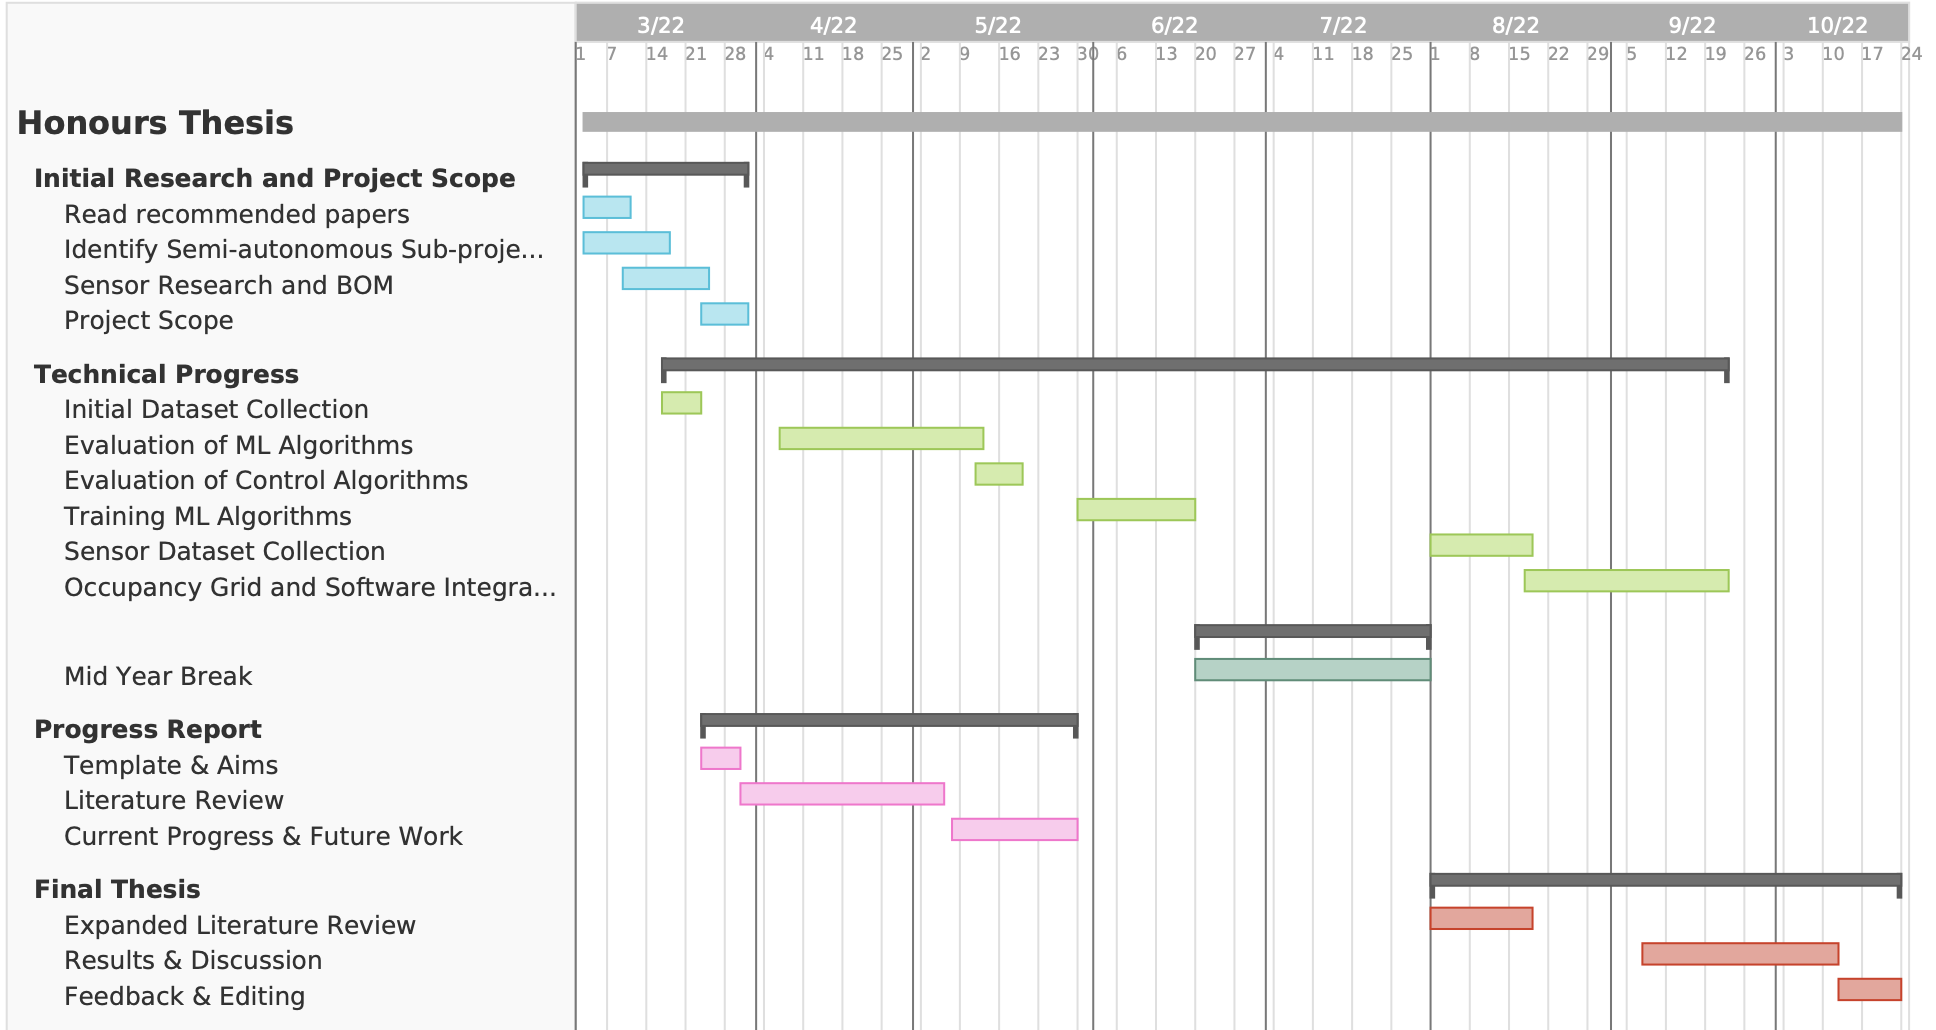
\includegraphics[width=\linewidth]{images/gantt_chart.png}
%    \caption{Gantt chart of thesis progress}
%    \label{fig:gantt_chart}
%\end{figure}
% TODO update Gantt chart

Code: \href{https://github.com/JakobWyatt/smart-wheelchair}{\underline{Github}}.
ZED Dataset: \href{https://curtin.sharepoint.com/:f:/r/sites/CurtinXGlide/Shared%20Documents/Navigation%20and%20Object%20Detection/ZED?csf=1&web=1&e=tTau9D}{\underline{Curtin X Glide (Smart Wheelchair)}} Teams channel.
Preliminary Dataset: \href{https://curtin.sharepoint.com/:v:/r/sites/CurtinXGlide/Shared%20Documents/Navigation%20and%20Object%20Detection/GoPro%20Dataset.mp4?csf=1&web=1&e=seLdRb}{\underline{(also hosted on teams)}}.


\end{document}
